\documentclass[11pt]{article}
\usepackage{amsthm}  
\usepackage{graphicx}
\usepackage[colorlinks,linkcolor=red]{hyperref} 
\usepackage{bigstrut,multirow,rotating} 
\usepackage{xcolor,array,tabularx,xurl,placeins}
\usepackage{booktabs}            
\usepackage{enumerate}
\usepackage{amsmath}
\usepackage{bbm}
\usepackage{amsfonts,amssymb}
\usepackage{appendix, subcaption}
\usepackage[numbers,sort&compress]{natbib}
\usepackage[a4paper, margin=3cm]{geometry}
\usepackage{authblk} % <-- Add this for multiple authors/affiliations
\usepackage[mathlines]{lineno}
\linenumbers
\setlength{\emergencystretch}{2em}
% --- Theorem styles -------------------------------------------------
\theoremstyle{plain}      % default: bold header + italic body
\newtheorem{theorem}{Theorem}[section]     % theorem 3.2, 3.3, … within section 3
\newtheorem{lemma}[theorem]{Lemma}         % share counter with theorems
\newtheorem{proposition}[theorem]{Proposition}
\newtheorem{corollary}[theorem]{Corollary}

\theoremstyle{definition} % bold header + upright body
\newtheorem{definition}[theorem]{Definition}
\newtheorem{remark}[theorem]{Remark}

% optional: custom qed symbol for proofs that end with equations
\renewcommand{\qedsymbol}{$\square$}

\title{Kernel Methods for the Computation of Quasi-Potentials in Stochastic Dynamical Systems}

\author[1]{Jonghyeon Lee\thanks{jlee9@caltech.edu}}
\author[1,5]{Boumediene Hamzi\thanks{boumediene.hamzi@gmail.com. Parts of this work were carried out while BH was a resident scholar at the Isaac Newton Institute for Mathematical Sciences, Cambridge, UK.}}
\author[2]{Yang Li \thanks{Corresponding author: liyangbx5433@163.com}}
\author[1]{Houman Owhadi\thanks{owhadi@caltech.edu}}
\author[3]{Umesh Vaidya\thanks{uvaidya@clemson.edu}}
\author[4]{Naiming Xie\thanks{xienaiming@nuaa.edu.cn}}

\affil[1]{Department of Computing and Mathematical Sciences, Caltech, CA, USA}
\affil[2]{School of Automation, Nanjing University of Science and Technology, Nanjing 210094, China}
\affil[3]{Department of Mechanical Engineering, Clemson University Clemson, SC, USA}
\affil[4]{Nanjing University of Aeronautics and Astronautics, Nanjing 210094, China}
\affil[5]{The Alan Turing Institute, London, UK}


\date{23 September 2026}

\begin{document}

  \maketitle

 
\begin{abstract}
We present a kernel framework for computing quasi-potentials of stochastic differential equations in the weak-noise regime. Direct scalar RKHS approximations and structured Koopman-coordinate surrogates combine Hamilton--Jacobi residual fitting with diffusion-dependent Riccati curvature at a stable equilibrium. Kernel-amplitude regularization and finite-dictionary selection provide complementary ways to control representation complexity. A conditional convergence theorem states the compactness, residual-control, and boundary comparison assumptions needed to identify the viscosity limit.

Numerical experiments recover two quartic reference potentials with polynomial kernels and reproduce a three-dimensional multiplicative-noise quadratic with a stable anchored kernel expansion. The three-dimensional fit achieves an RMSE of $1.35\times10^{-9}$ on an $8000$-point grid at $N=200$. Independent tests, multiple training seeds for the two-dimensional systems, and a structured eight-dimensional experiment assess accuracy and computational cost. A comparison with restricted quadratic Koopman representations identifies approximation bias associated with transformed diffusion. All numerical results are accompanied by code, fitted coefficients, and native vector figures.
\end{abstract}

\section{Introduction}
\label{intro}
Noise-induced transitions and rare escape phenomena are ubiquitous in physical, chemical, biological, and engineering systems \cite{horsthemke1984noise, zhu2003first}. The Freidlin-Wentzell large deviation theory serves as a fundamental framework for analyzing rare events driven by weak noise \cite{Freidlin2012, 10.1214/07-AOP362, dean2009splitting, huisinga2003extracting, lu2017gaussian}. Central to this theory is the concept of the action functional, which quantifies the likelihood of trajectories deviating from deterministic paths. The quasi-potential, defined as the infimum of the action functional, lies at the heart of large deviation theory. It characterizes the probability of a stochastic system fluctuating into a neighborhood of a specific state and governs key quantities such as mean first exit times and stationary distributions.

Despite its importance, computing the quasi-potential remains challenging. Traditional approaches can be categorized into three classes. Action Plot Methods \cite{beri2005solution}: These methods parameterize trajectories by integrating along unstable manifolds in the extended Hamiltonian phase space, starting from a small circle near a fixed point until exiting the basin of attraction. While effective for obtaining quasi-potential values along parameterized paths, they fail to establish a direct relationship between the quasi-potential and spatial coordinates. Geometric Minimum Action Method (GMAM) \cite{heymann2008geometric}: As a representative of string methods \cite{grafke2019numerical, zhou2008adaptive, cameron2011string, weinan2004minimum}, GMAM iteratively identifies the most probable path between a fixed point and a target state. However, it computes the quasi-potential only at discrete endpoints, lacking global structure. Ordered Upwind Method (OUM) \cite{cameron2012finding, dahiya2018ordered}: By discretizing the phase space and propagating quasi-potential values outward from fixed points, OUM achieves global quasi-potential reconstruction. Yet, its computational efficiency remains limited, especially in high-dimensional systems.

Recent advances in computational power and artificial intelligence have spurred the application of machine learning to stochastic dynamics. Techniques such as sparse regression \cite{Boninsegna2018, YangLi2020a}, Koopman operators \cite{EDMD, SKO3}, and neural networks \cite{XiaoliChen} have been leveraged for data-driven modeling of stochastic systems. In addition, some machine learning methods are also proposed to solve the problem of noise-induced transitions such as computing the most probable paths \cite{li2021machine, wei2022optimal} and the mean first exit times \cite{li2024deep}. Notably, Lin et al. \cite{lin2022data} proposed neural network-based frameworks to compute quasi-potentials for stochastic dynamical systems with additive Gaussian noise, while Li et al. \cite{li2022machine} developed physics-informed neural networks (PINNs) to compute quasi-potentials by solving Hamilton-Jacobi equations.

Among machine learning paradigms, kernel methods stand out due to their strong nonlinear representation capabilities and computational efficiency. Notably, reproducing kernel Hilbert spaces (RKHS) \cite{CuckerandSmale} have established solid mathematical foundations for the analysis of  dynamical systems \cite{BH4, yk1, bhcm11,bhcm1, lyap_bh, bh_sparse_kfs, BHPhysicaD, hamzi2019kernel, bh2020b,SKO3,ALEXANDER2020132520,bh12,bh17,hb17,mmd_kernels_bh, hamzipaillet,jalalian_deds_2023,lee2024note, hamzi2025kernel_lions, bittracher2021dimensionality} and surrogate modeling (cf.\ \cite{santinhaasdonk19} for a survey) as well as analyzing neural networks \cite{smirnov2022mean}. The idea of combining multiple kernels by learning a weighted mixture is known as \emph{multiple kernel learning} (MKL) \cite{lanckriet2004learning, bach2004multiple} and has been studied extensively in the machine learning literature. Our approach is related to MKL in that we learn a sparse convex combination of base kernels, but it differs in that the objective couples kernel selection with PDE residual minimization and curvature matching, rather than regression or classification loss.

\paragraph{Position relative to existing approaches.}\label{sec:positioning}
Kernel collocation and Gaussian-process methods provide smooth representations, derivative evaluation, and nonlinear PDE residual fitting \cite{Chen2021}. Physics-informed quasi-potential methods impose the Hamilton--Jacobi equation \cite{li2022machine,lin2022data}, while kernel Koopman methods approximate dynamical eigenfunctions and spectra \cite{Williams2015}. The present contribution couples a diffusion-dependent Riccati curvature target with direct scalar and Koopman-coordinate kernel surrogates, and specifies their distinct approximation properties. The Riccati term supplies local nontrivial geometry; global viscosity selection requires further conditions. Koopman coordinates give a structured nonnegative parametrization and linear inner transport fits, but their benefit over direct scalar RKHS fitting is problem dependent. Section~\ref{sec:koopman-role} explains this distinction, and Appendix~\ref{app:additional} provides a controlled comparison. Section~\ref{examples} studies two- and three-dimensional systems. Neither the meshfree representation nor those examples establishes general high-dimensional scalability.

In this work, we present a kernel-based algorithm for quasi-potential computation. The structure of this paper is as follows: Section~\ref{qpsec} introduces the definition and properties of the quasi-potential. Section~\ref{methsec} details the proposed kernel-driven methodology. Numerical examples in Section~\ref{examples} examine reconstruction accuracy and computational limitations, followed by concluding remarks.



%\section{Quasi-potential}

%Stochastic dynamical systems of the form
%\begin{equation}
%  dx_t = b(x_t) dt + \sqrt{\varepsilon}\,\sigma(x_t) dB_t
%\end{equation}
%model various phenomena where deterministic dynamics are influenced by noise. Here, \(\varepsilon\) is small, indicating weak noise, and \(B_t\) is a standard Brownian motion. The system tends to dwell near stable fixed points of the deterministic dynamics, occasionally making transitions due to noise.

%A key tool to study such transitions is the \emph{quasi-potential} \(V(x)\), which quantifies the most probable path of escape and transition probabilities. When the noise is weak, the stationary distribution takes the WKB form:
%\begin{equation}
%  p_s(x) \sim C(x)\,\exp(-\varepsilon^{-1} V(x))
%\end{equation}
%where \(V(x)\) solves a Hamilton-Jacobi equation (HJE):
%\begin{equation}
%  H(x, \nabla V) = b(x)^T \nabla V + \tfrac{1}{2} \nabla V^T a(x) \nabla V = 0
%\end{equation}
%with \(a(x) = \sigma(x) \sigma(x)^T\).


 


 

\setcounter{equation}{0}
\section{Quasi-Potential and the Wentzel--Kramers--Brillouin Approximation in Stochastic Dynamical Systems} \label{qpsec}

In this section, we examine dynamical systems governed by state variables \( x_t \in \mathbb{R}^n \), evolving under the influence of Gaussian white noise with low intensity. The dynamics are described by the stochastic differential equation:
\begin{equation}
\label{sde}
dx_t = b(x_t)\,dt + \sqrt{\varepsilon}\,\sigma(x_t)\,dB_t,
\end{equation}

where $B_t \in \mathbb{R}^n$ denotes an $n$-dimensional standard Brownian motion, and $\varepsilon$ is a small positive parameter quantifying the noise strength. The function $b(x) \in \mathbb{R}^n$ represents the deterministic drift term, which we assume has continuously differentiable derivatives. The diffusion coefficient is given by the matrix $a(x) = \sigma(x)\sigma(x)^\top$, where we assume $a(x)$ is uniformly positive definite on $\Omega$ (ensuring non-degeneracy of the noise).

We suppose $\bar{x}$ is an \textbf{asymptotically stable and hyperbolic} fixed point of the associated deterministic system, that is, $b(\bar{x}) = 0$ and all eigenvalues of its linearization matrix $J = \nabla b(\bar{x})$ have \textbf{strictly negative real parts}, i.e., $\text{Re}(\lambda_i) < 0$ for all $i = 1,\ldots,n$. This ensures asymptotic stability in the sense that trajectories starting near $\bar{x}$ converge to $\bar{x}$ exponentially in time. Under additional global confinement and recurrence assumptions, the perturbed process admits a stationary density $p_s(x)$; local stability alone does not imply this global property. In the regime of weak noise ($\varepsilon \ll 1$), this stationary distribution admits a Wentzel--Kramers--Brillouin (WKB)-type asymptotic approximation (see \cite{chen2017singularities,li2022machine,smelyanskiy1997topological}):
\begin{equation}
\label{WKB}
p_s(x) \sim C(x)\, \exp\left\{-\varepsilon^{-1} V(x)\right\},
\end{equation}
where \( C(x) \) is a slowly varying prefactor and \( V(x) \) is the quasi-potential function, characterizing the exponential decay rate of the probability density. This form is termed a \emph{WKB-type approximation} named after the WKB method in quantum mechanics, where solutions in the semiclassical limit \( \hbar \to 0 \) take the form \( \psi(x) \sim A(x)\exp\{i S(x)/\hbar\} \). In both contexts, the exponential term dominates and captures the leading-order behavior, while the prefactor varies more slowly. In stochastic systems, the small parameter \( \varepsilon \) appears in the exponent, leading to sharp concentration of the probability distribution around stable points as \( \varepsilon \to 0 \). The quasi-potential \( V(x) \) acts as an effective potential or energy landscape, quantifying the cost of rare fluctuations. The symbol ``\( \sim \)'' denotes logarithmic equivalence, meaning that
\[
\lim_{\varepsilon \to 0}-\varepsilon\log p_s(x)=V(x),
\]
after compatible normalization and in the relevant single-attractor asymptotic setting. In a multistable problem, the stationary rate function and the action value relative to one attractor must be distinguished.

The concept of the quasi-potential originates from large deviation theory \cite{Freidlin2012}. It is defined via a variational principle involving the Freidlin--Wentzell action functional \( S_T[\phi] \), formulated over continuous trajectories \( \phi(t) \) that connect a stable fixed point \( \bar{x} \) to a target point \( x \). Specifically, the quasi-potential is given by the nested infimum:
\begin{equation}
\label{quasip}
V(x) \equiv \inf_{T > 0} \inf_{\phi \in AC([0, T])} \left\{ S_T[\phi] \,:\, \phi(0) = \bar{x},\; \phi(T) = x \right\},
\end{equation}
where \(AC([0,T])\) denotes absolutely continuous paths; the action is infinite outside its admissible path class. The action functional \( S_T[\phi] \), fundamental in the large deviation framework, is given by
\begin{equation}
\label{actionf}
S_T[\phi] = \int_0^T L(\phi(t), \dot{\phi}(t))\,dt,
\end{equation}
with the Lagrangian \( L(\phi, \dot{\phi}) \) for the stochastic differential equation \eqref{sde} defined as follows
\begin{equation}
\label{Lagran}
L(\phi, \dot{\phi}) = \frac{1}{2} \left[ \dot{\phi} - b(\phi) \right]^{\!\!T} a^{-1}(\phi) \left[ \dot{\phi} - b(\phi) \right].
\end{equation}

This action functional quantifies the cost of deviations from the deterministic path and plays a central role in describing the asymptotic probability of rare events. In particular, for a fixed trajectory \( \phi(t) \), the probability that the stochastic process \( x_t \) remains within a small tube around \( \phi(t) \) over the time interval \([0, T]\) satisfies the large deviation estimate:
\begin{equation}
\label{LDP}
\mathbb{P}_{x_0} \left\{ \sup_{t \in [0, T]} \left| x_t - \phi(t) \right| < \delta \right\} \sim \exp\left\{ -\varepsilon^{-1} S_T[\phi] \right\},
\end{equation}
for small \( \delta > 0 \), illustrating that the action functional governs the exponential rate of decay of such pathwise probabilities.

Note that the stationary probability distribution satisfies the time-independent Fokker--Planck equation 
\[ \mathcal{L}p_s(x) = - \sum_{i=1}^n \frac{\partial}{\partial x_i}\bigl(b_i(x)p_{s}(x)\bigr) + \frac{\varepsilon}{2}\sum_{i,j=1}^n \frac{\partial^2}{\partial x_i \partial x_j}\bigl(a_{ij}(x)p_{s}(x)\bigr) = 0, \]
where \( \mathcal{L} \) is the Fokker--Planck operator. Substituting the WKB ansatz \eqref{WKB} into this equation and collecting the leading-order terms in \( \varepsilon \) yields the Hamilton--Jacobi equation:
\begin{equation}
\label{HJE}
H(x, p) \equiv b^{T}p + \frac{1}{2} p^{T}ap = 0, \quad p \equiv \nabla V (x),
\end{equation}
which is a first-order nonlinear partial differential equation for the quasi-potential \( V \). It is observed that this Hamiltonian is the Legendre transform of the Lagrangian \eqref{Lagran}. According to the definition \eqref{quasip}, the quasi-potential at the fixed point satisfies \( V(\bar{x}) = 0 \). Since the quasi-potential function attains minimal value at the stable fixed point, the gradient of the quasi-potential is also zero at the stable point, i.e., $\nabla V(\bar{x}) =0$.

If \( b(x) = -\nabla U(x) \) (i.e., a gradient system) and \( a(x) = I \) (i.e., additive noise), then within the relevant attraction basin the quasi-potential is \(V(x)=2[U(x)-U(\bar x)]\), under the usual connecting-path assumptions. In this special case, the quasi-potential admits an analytical expression.

Assume that the second-order approximation of the quasi-potential function at the fixed point \( \bar{x} \) is given by
\[
\begin{aligned}
V(x) & \approx V(\bar{x}) + \nabla V(\bar{x}) (x - \bar{x}) + \frac{1}{2} (x - \bar{x})^T \nabla^2 V(\bar{x}) (x - \bar{x}) \\
& = \frac{1}{2} (x - \bar{x})^T Z (x - \bar{x}),
\end{aligned}
\]
where \( Z = \nabla^2 V(\bar{x}) \). Consequently, its gradient is approximated as
\[
\nabla V(x) \approx Z (x - \bar{x}).
\]
Substituting the gradient approximation into the Hamilton--Jacobi equation (\ref{HJE}) yields
\begin{equation}\label{HJE2}
b(x)^T Z (x - \bar{x}) + \frac{1}{2} (x - \bar{x})^T Z^T a(x) Z (x - \bar{x}) \approx 0.
\end{equation}
Near the fixed point, we also approximate the drift $b(x)$ and the diffusion $a(x)$ as
\[
b(x) \approx F(x-\bar{x}), \ a(x) \approx A,
\]
where $F \equiv \nabla b(\bar{x}), A \equiv a(\bar{x})$. Substituting the linearized $b(x)$ and $a(x)$ into Eq. (\ref{HJE2}), we have
\begin{equation}\label{HJE3}
(x - \bar{x})^T (F^TZ + \frac{1}{2} Z^TAZ) (x - \bar{x}) \approx 0.
\end{equation}
Note that it is equivalent to the following equation.
\begin{equation}\label{HJE4}
(x - \bar{x})^T (F^TZ + ZF + Z^TAZ) (x - \bar{x}) \approx 0.
\end{equation}
Since the matrix $F^TZ + ZF + Z^TAZ$ is a symmetric matrix, it must be diagonalizable. Due to the arbitrariness of $x - \bar{x}$, the eigenvalues of the matrix must all be 0. That is, each element of the matrix is 0. Therefore, the Hessian matrix \( Z = \nabla^2 V(\bar{x}) \) satisfies the algebraic Riccati equation:
\begin{equation}\label{HJE5}
 F^TZ + ZF + Z^TAZ= 0
\end{equation}
or the equivalent form:
\begin{equation}
\label{Riccati}
FZ^{-1} + Z^{-1}F^T + A = 0.
\end{equation}

The principal challenge in computing the quasi-potential from the PDE \eqref{HJE} lies in avoiding trivial solutions. To address this, we employ kernel methods to solve the PDE \eqref{HJE}, and use equation \eqref{Riccati} to impose that the Hessian of \( V \) at the origin coincides with the matrix \( Z \) solving \eqref{Riccati}.

It is worth emphasizing that the quasi-potential plays a pivotal role not only in large deviation theory but also in stochastic dynamics, as it is linked to various physical quantities. For example, the expected time to exit the domain of attraction of a fixed point---known as the mean exit time---is exponentially determined by the minimum of the quasi-potential on the boundary of the domain. The exit location distribution and the invariant measure can also be approximated based on the quasi-potential. Furthermore, once the quasi-potential function is known, the most probable transition path connecting two steady states can be derived from the quasi-potential. Typically, the most probable path passes through a saddle point, with the latter half of the trajectory beyond the saddle point following its unstable manifold toward the destination steady state. The first half of the path is obtained by solving the equation \begin{equation}\label{mppcomp}
\dot{x} = b(x) + a(x) \nabla V(x).
\end{equation}
The boundary conditions are $x(-\infty)=\bar{x}$ and $x(\infty)=x_{sa}$, where $x_{sa}$ denotes the saddle point. In practice, Equation (\ref{mppcomp}) is obtained by substituting $p= \nabla V(x)$ into the state equation $\dot{x} = b(x) + a(x)p$ of the Hamiltonian system corresponding to the Hamilton-Jacobi Equation (\ref{HJE}). Therefore, the most probable path is the projection of a heteroclinic orbit in the $2n$-dimensional Hamiltonian phase space onto the $n$-dimensional state space. For further properties of the quasi-potential, see \cite{Freidlin2012}. \begin{remark}
When $\varepsilon = 0$ (i.e. when there is no noise), our work will reduce to constructing the Lyapunov function for the unforced system $\dot{x} = b(x)$ \cite{giesl2019approximation, lee2024note}
\end{remark}


\section{Method for Approximating the Quasi-Potential}\label{methsec}

We consider both direct scalar kernel approximations and a structured spectral representation. The latter exploits the Koopman operator; its construction is developed first, and the direct finite-feature implementation is given in Section~\ref{sec:direct-implementation}. Specifically, we construct eigenfunctions \( \varphi_i(x) \) satisfying the linear advection-type partial differential equations:
\begin{equation}
\nabla \varphi_i(x) \cdot b(x) = \lambda_i \varphi_i(x), \quad \varphi_i(\bar{x}) = 0, \quad \nabla \varphi_i(\bar{x}) = \ell_i,
\end{equation}
where \( \lambda_i \) are eigenvalues of the linearization \( J = \nabla b(\bar{x}) \) at the fixed point \( \bar{x} \), and \(\ell_i\) are left eigenvectors, \(J^\top\ell_i=\lambda_i\ell_i\). Standard basis vectors give this normalization only in suitable coordinates. Complex conjugate modes are handled through their real and imaginary parts; smooth independent eigenfunctions on an entire basin require additional dynamical assumptions. These eigenfunctions correspond to the Koopman eigenfunctions associated with the equilibrium dynamics and encode local geometric and dynamical information such as the structure of stable and unstable manifolds.

Let $\Phi=(\varphi_1,\ldots,\varphi_n)^\top$ in a real coordinate representation, and let $S$ be the invertible matrix of prescribed gradients at $\bar x$ (rows $\ell_i^\top$, or corresponding real blocks). We define
\begin{equation}\label{eq:vmid}
 V_{\mathrm{mid}}(x)=\tfrac12\Phi(x)^\top P_{\mathrm{mid}}\Phi(x),
 \qquad P_{\mathrm{mid}}=S^{-\top}P_{\mathrm{loc}}S^{-1},
\end{equation}
where $P_{\mathrm{loc}}$ is the positive-definite physical Riccati Hessian. This matrix is symmetric and includes the diffusion information. If the value and gradient normalizations of $\Phi$ hold exactly, the Hessian of $V_{\rm mid}$ is exactly $P_{\rm loc}$; the curvature penalty remains useful for approximate enforcement. A similarity transform of eigenvalues alone is not a general formula for this Hessian.

To represent \( \varphi_i(x) \), we employ a data-driven kernel-based ansatz:
\begin{equation}\label{phiix}
\varphi_i(x) = \sum_{p=1}^N \alpha_p^{(i)}\,k_\beta(x, x_p) + (x - \bar{x}) \cdot \ell_i,
\end{equation}
where the point set \( \{ x_p \}_{p=1}^N \) denotes the collocation set which is used for training, and \( k_\beta(x, t) \) is $k_\beta=\sum_j\beta_j^2k_j$, a convex combination of base kernels with nonnegative amplitudes $\beta$ satisfying $\sum_j\beta_j^2=1$. This kernel formulation ensures flexibility and regularization, and it circumvents the need to construct the Koopman operator explicitly.

The coefficients $\alpha_p$ are determined by a regularized finite-section collocation fit. A derivative-loss representer theorem involves the corresponding derivative functionals and does not by itself identify the quadratic eigenfunction surrogate with a scalar RKHS minimizer.   
To determine the coefficients $\alpha^{(i)} = (\alpha^{(i)}_1,\dots,\alpha^{(i)}_N)$,
we enforce the Koopman eigenfunction equation at the collocation points.
Specifically, for each $i=1,\dots,n$, we impose the conditions
\[
\varphi_i(\bar x)=0, \qquad
\nabla\varphi_i(\bar x)=\ell_i,
\]
together with the PDE constraint
\[
\nabla\varphi_i(x_p)\cdot b(x_p)
= \lambda_i\,\varphi_i(x_p),
\qquad p=1,\dots,N.
\]
Substituting the RKHS ansatz (\ref{phiix}) into these conditions yields a linear
system for the coefficients $\alpha^{(i)}$, which we solve in a
regularized least--squares sense:
\begin{equation}
    \label{eqn:alpha_eqn}
\min_{\alpha^{(i)}} \;
\sum_{p=1}^N 
\left(
\nabla\varphi_i(x_p)\cdot b(x_p)
- \lambda_i\,\varphi_i(x_p)
\right)^2
\;+\;
\eta\,\|\varphi_i\|_{\mathcal{H}_k}^2,
\qquad 
\|\varphi_i\|_{\mathcal H_k}^2
= \alpha^{(i)T} G_\beta \alpha^{(i)}.
\end{equation}
Here $(G_\beta)_{pq}=k_\beta(x_p,x_q)$ is the kernel Gram matrix.
The solution of this regularized linear system provides the coefficients
$\alpha^{(i)}$ used to construct $\Phi(x)$ and the quasi-potential
surrogate $V_{\rm mid}(x)$.


\begin{remark}[RKHS norm and the linear correction term]
The ansatz~\eqref{phiix} decomposes $\varphi_i$ into an RKHS part $\sum_p \alpha_p^{(i)} k_\beta(x,x_p)$ and a fixed linear term $(x-\bar{x})\cdot\ell_i$. The RKHS norm $\|\varphi_i\|_{\mathcal{H}_k}^2 = \alpha^{(i)T}G_\beta\alpha^{(i)}$ penalizes only the learnable kernel component, not the linear correction. This is intentional: the linear term is analytically prescribed by the boundary condition $\nabla\varphi_i(\bar{x})=\ell_i$ and carries zero free parameters, so it should not be regularized. Penalizing it would bias the solution away from the exact local linearization.
\end{remark}


To determine optimal kernel weights \( \beta \), we minimize the following regularized loss function, where $P_{\text{loc}} \in \mathbb{R}^{n \times n}$ denotes the local curvature target matrix---specifically, the positive-definite solution of the algebraic Riccati equation~\eqref{Riccati} evaluated at $\bar{x}$:

\begin{align}\label{eq:composite_loss}
L(\beta) = & \underbrace{\sum_p \left[ b^{T}(x_p)\nabla V_{\text{mid}}(x_p) + \frac{1}{2} \nabla V_{\text{mid}}(x_p)^{T}a(x_p)\nabla V_{\text{mid}}(x_p)\right]^2}_{L_{\text{HJ}}}
+ \gamma \underbrace{\|\nabla^2 V_{\text{mid}}(\bar{x}) - P_{\text{loc}}\|_F^2}_{L_{\text{curv}}} \notag \\
& + \lambda_1 \sum_j |\beta_j| + \eta \sum_i \|\varphi_i\|_{\mathcal{H}_k}^2,
\end{align}
subject to the constraints \( \beta_j \ge 0 \) and \( \sum_j \beta_j^2 = 1 \). Here $\| \cdot \|_F$ denotes the Frobenius norm. The first term $L_{\text{HJ}}$ enforces consistency with the Hamilton--Jacobi structure; the second term $L_{\text{curv}}$ aligns the local curvature of the approximation with that of the Riccati solution at $\bar{x}$. The remaining terms promote sparsity and RKHS regularity.

\paragraph{Kernel amplitudes versus mixture weights.}\label{sec:amplitudes}
We use nonnegative amplitudes $\beta_j$ with $\sum_j\beta_j^2=1$ and define the actual mixture weights as $w_j=\beta_j^2$. Thus $k_\beta=\sum_j\beta_j^2k_j$ is a convex kernel combination, while the sparsity penalty is applied to the amplitudes. It is nonconstant:
\[
 1\leq\sum_j\beta_j\leq\sqrt L.
\]
Its minimum is attained by a single active amplitude, so it encourages concentrated mixtures; it does not guarantee that a nonconvex optimizer finds a particular sparse model. In contrast, an $\ell_1$ penalty on simplex weights $w_j\geq0$, $\sum_jw_j=1$ is constant and has no sparsifying effect. The distinction is essential. Pruning small weights or amplitudes is an additional heuristic, followed by renormalization and refitting. In a single-component model the active amplitude and its weight both equal one. The discrete polynomial-degree selection used in Section~\ref{examples} is specified separately from continuous mixture optimization.

\paragraph{Algorithmic structure.}
In practice, the computation proceeds in two stages. For a fixed choice of kernel weights $\beta$, the coefficients $\alpha^{(i)}$ are obtained by solving the regularised linear systems (\ref{eqn:alpha_eqn}), yielding the Koopman eigenfunction approximations $\varphi_i$ and hence $\Phi(x)$.  In a second, outer optimisation loop, the kernel mixture coefficients $\beta$ are updated by minimising the composite loss (\ref{eq:composite_loss}), while at each iteration the functions $\varphi_i$ are recomputed from the updated kernel $k_\beta$.  This bi-level structure separates the inner transport objective from the outer HJ objective. The inner and outer objectives play different roles when comparing the hybrid construction with a direct scalar fit.


\paragraph{Kernel dictionary.}
The general framework admits a dictionary combining Gaussian radial basis function (RBF) kernels and polynomial kernels. Section~\ref{examples} examines polynomial components, and Appendix~\ref{app:additional} evaluates Gaussian kernels. This choice is motivated by complementary approximation properties: RBF kernels excel at local interpolation and capturing rapid variations near critical points, while polynomial kernels naturally encode global algebraic structure characteristic of quasi-potentials. RBF+polynomial dictionaries have demonstrated robust performance across diverse dynamical-systems benchmarks \cite{hamzi2021learning}. Applied to the normalized amplitudes specified above, the $\ell_1$ term in the composite loss~\eqref{eq:composite_loss} encourages concentrated kernel mixtures, in the spirit of MKL \cite{lanckriet2004learning, bach2004multiple}: small components may be suppressed during fitting and removed by the stated pruning rule; exact sparse recovery is not guaranteed. In principle, the framework can accommodate much larger and more diverse kernel dictionaries; in \cite{bh_sparse_kfs} the same $\ell_1$-based sparsification mechanism was used with an extensive kernel library to learn 132 chaotic dynamical systems. The methodology naturally extends to other kernel families (e.g., Mat\'ern, rational quadratic, or domain-specific kernels) when more complex functional structures are anticipated.


\paragraph{Role and limitations of the Koopman representation.}\label{sec:koopman-role}
A direct comparator is $V_D(x)=\tfrac12(x-\bar x)^\top P_{\rm loc}(x-\bar x)+f_k(x)$, where the kernel correction can be constrained to have zero value, gradient, and Hessian at $\bar x$. Such a scalar model can minimize the same HJ residual without first learning eigenfunctions. Both methods permit analytic differentiation. The spectral model instead fits $n$ transport equations, provides nonnegativity when $P_{\rm mid}\succ0$, and supplies dynamical coordinates that may be reused in other tasks. These are structural advantages, not a proof of better accuracy or lower total cost.

In real coordinates with $D\Phi(\bar x)=I$, suppose $D\Phi\,b=F\Phi$ exactly and set $V_K=\tfrac12\Phi^\top P\Phi$. Then
\begin{equation}\label{eq:transformed-diffusion}
 H(x,\nabla V_K)=\tfrac12\Phi^\top
 \bigl(F^\top P+PF+P a_\Phi(x)P\bigr)\Phi,
 \quad a_\Phi=D\Phi\,a\,D\Phi^\top.
\end{equation}
The transformed diffusion is generally state dependent, so local Riccati matching does not make this expression vanish everywhere. For example, $b(x)=-x(1+x^2)$, $a(x)=1+x^2$ has $V(x)=x^2$ and the normalized eigenfunction $\varphi=x/\sqrt{1+x^2}$ with eigenvalue $-1$. The quadratic spectral candidate is $V_K=\varphi^2=x^2/(1+x^2)$, with
\[
 H(x,V_K')=-\frac{2x^4(2+x^2)}{(1+x^2)^3}.
\]
It matches the correct Hessian at zero but is not the quasi-potential. Thus a finite quadratic eigenfunction representation can have approximation bias even with exact eigenfunctions. Appendix~\ref{app:additional} compares a direct scalar correction and this restricted spectral construction using common data and curvature constraints; the tests favor the direct construction within these specified model classes. The Gaussian-kernel models in that comparison complement the polynomial-kernel experiments in Section~\ref{examples}.

\paragraph{Theoretical guarantee and solution selection.}\label{sec:solution-selection}
The composite loss \eqref{eq:composite_loss} couples a Hamilton--Jacobi residual, a regularizer, and a Riccati-curvature term. These ingredients address PDE fit, capacity, and local geometry, respectively. A convergence statement must also identify the action-selected solution. Strict convexity of $H(x,\cdot)$ does not supply this selection: for $b(x)=-x$ and $a=1$, both $u=0$ and $u=x^2$ solve the HJ equation and satisfy $u(0)=0$. Curvature matching excludes the constant candidate locally but does not by itself establish global uniqueness. We therefore state the comparison, compactness, and residual-control requirements explicitly, following viscosity stability \cite{Crandall1992}.

\begin{theorem}[Conditional consistency with Riccati-curvature matching]\label{thm:consistency-curvature}
Let $D\subset\mathbb R^d$ be a bounded domain with compact closure. Suppose $b,a$ are continuous, $a$ is uniformly positive definite, and compatible continuous boundary data $g$ select the desired restriction $V$ of the quasi-potential through
\[
H(x,\nabla V)=0\quad\text{in }D,\qquad V=g\quad\text{on }\partial D.
\]
Assume that this boundary-value problem has a continuous viscosity solution and a comparison principle in the relevant bounded continuous class. Let $V_N\in C^1(\overline D)$ be a sequence of kernel-based surrogates satisfying:
\begin{enumerate}
\item $V_N$ are uniformly bounded and equicontinuous on $\overline D$;
\item $\|V_N-g\|_{L^\infty(\partial D)}\to0$;
\item for $r_N(x)=H(x,\nabla V_N(x))$, the collocation sets $X_N$ have fill distance $h_N\to0$, the residuals have a common modulus of continuity $\omega$, and $\max_{x_p\in X_N}|r_N(x_p)|\to0$.
\end{enumerate}
Then $V_N\to V$ uniformly on $\overline D$, and hence in $L^2(\rho)$ for every probability measure $\rho$ on that closure.

If, in addition, the functions are $C^2$ near $\bar x$ and satisfy
$\|D^2V_N(\bar x)-P\|_F\to0$, their equilibrium curvature converges to $P$, where
\[
 b'(\bar x)^\top P+P b'(\bar x)+P a(\bar x)P=0,\qquad P\succ0.
\]
Gradient convergence requires additional compactness: if $V\in C^1$ and $\{\nabla V_N\}$ is relatively compact in $C(K)$ on every compact $K\Subset D$, then $\nabla V_N\to\nabla V$ uniformly on such $K$. None of these compactness or solution-selection conditions follows solely from small empirical loss.
\end{theorem}

\begin{remark}[Notation and empirical objective]
$V_N$ denotes a sample-dependent approximation, $V_{\rm mid}$ the quadratic Koopman surrogate, and $V_h$ or $V_{\rm quad}$ particular numerical reconstructions. Write $\mathcal R(\Phi,\beta)$ for the nonnegative regularizer of the learnable kernel components and amplitudes. The normalized empirical objective is
\begin{equation}\label{eq:empirical-loss}
\begin{aligned}
\mathcal L_{N,\lambda,\gamma}(\Phi,\beta)
={}&\frac1N\sum_{p=1}^N H(x_p,\nabla V_{(\Phi,\beta)}(x_p))^2\\
&+\gamma\|D^2V_{(\Phi,\beta)}(\bar x)-P\|_F^2
+\lambda\mathcal R(\Phi,\beta).
\end{aligned}
\end{equation}
The theorem concerns sequences meeting its stated conditions, not arbitrary local or global minimizers of this nonconvex objective. Its boundary data are an additional solution-selection condition, not the single point constraint $V_N(\bar x)=0$ used in a local fit.
\end{remark}

\begin{proof}[Proof of Theorem~\ref{thm:consistency-curvature}]
\textbf{Step 1: Finite representations and their scope.}
Kernel section expansions provide the numerical parametrizations. In an optimization over a scalar RKHS with bounded derivative evaluation functionals, a generalized representer theorem uses kernel derivatives associated with those functionals \cite{Chen2021}. A quadratic form in RKHS eigenfunctions is not automatically the same scalar RKHS minimizer. The convergence argument below uses the regularity and compactness stated in the theorem, rather than making that identification. In particular, bounded second-derivative evaluation functionals require more kernel regularity than merely assuming that the kernel is $C^2$.

\medskip\noindent\textbf{Step 2: Population risk and curvature.}
For any candidate $u$, define
\[
 R(u)=\mathbb E_\rho[H(X,\nabla u(X))^2],\qquad
 C(u)=\|D^2u(\bar x)-P\|_F^2.
\]
The regularized population objective is $R(u)+\gamma C(u)+\lambda\mathcal R(u)$. Zero residual does not imply uniqueness, and a regularizer need not vanish at the true solution. Uniqueness of the viscosity limit will instead follow from the assumed boundary-value comparison principle.

\medskip\noindent\textbf{Step 3: What empirical optimality gives.}
Let $\widehat R_N(u)=N^{-1}\sum_p H(x_p,\nabla u(x_p))^2$. If $u_N$ minimizes the regularized empirical objective up to tolerance $\delta_N\geq0$, comparison with any admissible $w_N$ gives
\begin{equation}\label{eq:excess-risk}
\begin{aligned}
\widehat R_N(u_N)+\gamma_N C(u_N)+\lambda_N\mathcal R(u_N)
\leq{}&\widehat R_N(w_N)+\gamma_N C(w_N)\\
&+\lambda_N\mathcal R(w_N)+\delta_N.
\end{aligned}
\end{equation}
All comparator regularization and optimization terms must be retained. This inequality explains the need for approximation and optimization control; it does not give a gradient-error bound. The comparison with kernel-ridge excess-risk analysis \cite{CaponnettoDeVito2007,SteinwartChristmann2008} is methodological, not a transfer of its rates to the nonlinear HJ loss.

\medskip\noindent\textbf{Step 4: From samples to a uniform residual.}
For each $x\in\overline D$, choose a nearest collocation point. The common modulus yields
\begin{equation}\label{eq:uniform-residual}
 \|r_N\|_{L^\infty(D)}
 \leq \max_{x_p\in X_N}|r_N(x_p)|+\omega(h_N)\longrightarrow0.
\end{equation}
This is a stronger requirement than $\widehat R_N(V_N)\to0$. For example,
$\max_p|r_N(x_p)|\leq\sqrt{N\widehat R_N(V_N)}$ gives the sufficient, but not necessary, condition $N\widehat R_N(V_N)\to0$ when combined with uniform residual regularity. A population-risk route would need a uniform generalization estimate and sufficient control of residual spikes; no such rate is asserted here.

\medskip\noindent\textbf{Step 5: Compactness.}
Uniform boundedness and equicontinuity give, by Arzel\`a--Ascoli, a uniformly convergent subsequence $V_{N_j}\to u$ on $\overline D$. The boundary assumption implies $u=g$ on $\partial D$. In particular, compactness is an independent hypothesis; kernel smoothness alone does not provide a uniform bound on fitted derivatives as regularization vanishes.

\medskip\noindent\textbf{Step 6: Viscosity identification.}
If a $C^1$ function $\phi$ touches $u$ from above at an interior point $x$, a small strictifying perturbation and uniform convergence produce local maxima of $V_{N_j}-\phi$ at $x_j\to x$. There,
\[
 \nabla V_{N_j}(x_j)=\nabla\phi(x_j),\qquad
 H(x_j,\nabla\phi(x_j))=r_{N_j}(x_j)\to0.
\]
Continuity of $H$ gives the subsolution inequality. The same argument with local minima gives the supersolution inequality. Thus $u$ is a viscosity solution with data $g$. Comparison identifies $u=V$. Every subsequential limit has this value, so the entire sequence converges uniformly and therefore in $L^2(\rho)$.

\medskip\noindent\textbf{Step 7: Hessian consistency.}
The additional curvature hypothesis gives the stated Hessian convergence directly. For a penalized fit it is sufficient that the attained nonnegative objective in \eqref{eq:empirical-loss} is $o(\gamma_N)$, because
\[
 C(V_N)\leq\mathcal L_{N,\lambda_N,\gamma_N}(V_N)/\gamma_N.
\]
Merely taking $\gamma_N\to0$ does not imply this conclusion. Exact curvature constraints are an alternative.

\medskip\noindent\textbf{Step 8: The additional gradient conclusion.}
Under the stated gradient compactness assumption, any subsequence has a further subsequence whose gradients converge uniformly on $K$ to some $q$. Integration against compactly supported test functions, together with uniform convergence of $V_N$, identifies $q$ as the distributional gradient of $V$, hence as $\nabla V$ when $V\in C^1$. Uniqueness of this limit gives convergence on every compact subset. No gradient convergence is asserted across a nonsmooth quasi-potential without further analysis.
\end{proof}

\paragraph{Interpretation of the assumptions.}
For a quasi-potential, the boundary or admissibility problem must select the action value in \eqref{quasip}. A truncated, punctured basin with compatible action data is one possible setting, provided its comparison principle is established. The local experimental fits do not establish those conditions and are therefore assessed through numerical diagnostics rather than claimed as instances of an unconditional consistency theorem. Likewise, the monotone-scheme theorem of Barles and Souganidis \cite{Barles1991} cannot be applied directly: monotonicity of the present nonlinear kernel least-squares scheme has not been proved. A fixed quadratic Koopman class need not be dense in the required derivative topology even when the scalar kernel is universal. These distinctions preserve the role of Riccati matching without equating local curvature with global solution selection.

The following corollary records the local Riccati condition for a smooth solution with a nondegenerate minimum. It is separate from the global viscosity-selection question.

\begin{corollary}[Local Consistency with the Hamilton--Jacobi Equation]\label{cor:localHJ}
Let $V \in C^{2}(\Omega)$ solve
\[
H(x,\nabla V(x))
=f(x)^\top \nabla V(x)
+\tfrac{1}{2}\nabla V(x)^\top a(x)\,\nabla V(x)=0,
\qquad V(\bar{x})=0,
\]
with $f=b$, $b\in C^1$, $a(\bar x)\succ0$, $Db(\bar x)$ Hurwitz, $\nabla V(\bar x)=0$, and $D^2V(\bar x)\succ0$. The positive-Hessian condition excludes the constant HJ solution.
Then the Hessian of $V$ at $\bar{x}$ equals the Riccati matrix $P$:
\[
D^{2}V(\bar{x})=P,
\]
where $P$ is the unique positive-definite solution to the algebraic Riccati equation
\[
b'(\bar{x})^\top P + P\,b'(\bar{x}) + P\,a(\bar{x})\,P=0.
\]
\end{corollary}

\begin{proof}
Near the equilibrium point $\bar{x}$, write the Taylor expansion
\[
V(x)=\tfrac{1}{2}(x-\bar{x})^\top Z(x-\bar{x})
+o\!\left(\|x-\bar{x}\|^{2}\right),
\qquad Z=D^{2}V(\bar{x}).
\]
Linearise the drift and diffusion at $\bar{x}$:
\[
f(x)=b'(\bar{x})(x-\bar{x})+o(\|x-\bar{x}\|),\qquad
a(x)=a(\bar{x})+o(1).
\]
Thus the gradient satisfies $\nabla V(x)=Z(x-\bar{x})+o(\|x-\bar{x}\|)$.
Insert these expansions into the Hamilton--Jacobi equation:
\[
H(x,\nabla V(x))=
f(x)^\top\nabla V(x)
+\tfrac{1}{2}\nabla V(x)^\top a(x)\,\nabla V(x)=0.
\]
Collecting second-order terms in $x-\bar{x}$ yields
\[
(x-\bar{x})^\top\!
\bigl(b'(\bar{x})^\top Z + Z b'(\bar{x})
+Z a(\bar{x})Z\bigr)(x-\bar{x})
+o\!\left(\|x-\bar{x}\|^{2}\right)=0.
\]
Since this holds for all $x$ near $\bar{x}$, the symmetric coefficient must vanish:
\[
b'(\bar{x})^\top Z + Z b'(\bar{x}) + Z a(\bar{x})Z =0.
\]
By standard results on algebraic Riccati equations (positive-definite $a(\bar{x})$ and stability of $b'(\bar{x})$), there is a unique positive-definite solution $P$ of this equation.
Since $Z\succ0$, multiplying by $Z^{-1}$ gives the uniquely solvable Lyapunov equation for $Z^{-1}$; hence $Z=P$ and $D^{2}V(\bar{x})=P$.
\end{proof}



\paragraph{Computational complexity, memory, and dimensional scope.}\label{sec:complexity-full}
Let $N$ be the collocation count, $M$ the number of centers ($M=N$ in a full section expansion), $n$ the state dimension, $L$ the dictionary size, and $T$ the number of outer kernel evaluations. For common radial kernels, constructing values and first derivatives costs $O(LNMn)$; retaining all derivative arrays uses $O(LNMn)$ storage. A single dense $N\times N$ Gram matrix requires $8N^2$ bytes in float64. The often-quoted $O(N^2n)$ is an assembly cost, not the cost of solving a dense system: factorization requires $O(N^3)$ time and $O(N^2)$ memory. Initial computation of the Riccati target through a dense Lyapunov solve costs $O(n^3)$.

For $n$ independent scalar eigenfunction fits with $M$ centers, dense least-squares work can be $O(n(NM^2+M^3))$ per kernel choice, in addition to assembly. Factorizations can sometimes be reused, but cannot generally be shared across distinct eigenvalues or updated kernels. Real block formulations for complex eigenpairs may require coupled solves. A generic fully coupled system has $Nn$ rows and $Mn$ columns: storing its design and normal matrices costs $O(NMn^2+M^2n^2)$, and forming/factoring normal equations can cost $O(NM^2n^3+M^3n^3)$. Exploiting spectral or block structure reduces this upper bound. The implementation in Appendix~\ref{app:additional} uses the coupled real form.

A direct scalar $M$-coefficient HJ fit has nonlinear least-squares steps costing approximately $O(NM^2+M^3)$, plus gradient/residual assembly. Dense diffusion contributes $O(Nn^2)$ matrix-vector work, excluding coefficient evaluation. For structured radial derivatives, evaluating a trained spectral potential and gradient at one point costs approximately $O(LMn^2+n^2)$, versus $O(LMn+n^2)$ for a scalar section expansion. Dense Taylor-Hessian contractions in the exact-curvature direct implementation of Appendix~\ref{app:additional} add $O(Mn^2)$ work per point. The outer selection loop repeats inner work $T$ times. Derivative workspaces, optimizer arrays, and validation evaluation must therefore be included in practical budgets.

Kernel sparsification reduces $L$ but does not by itself reduce $N$ or $M$. Nor does algebraic dependence on dimension in an individual operation remove the sample-coverage burden: a tensor grid with $q$ points per coordinate has $N=q^n$. The examples in Section~\ref{examples} cover dimensions two and three. Appendix~\ref{app:additional} studies a structured eight-dimensional system and reports timing and storage measurements; these tests do not establish dimension-independent scalability. Sparse centers, structured linear algebra, and reduced-order models are possible future improvements, rather than established performance guarantees of the current method.

\subsection{Direct scalar implementation and stable finite features}\label{sec:direct-implementation}
The HJ equation can be fitted directly in a scalar kernel space while retaining the same local Riccati information. This option separates potential approximation from the additional transport restriction imposed by a Koopman-coordinate model. Let $y=x-\bar x$. For polynomial kernels of degree $r$, use the finite-feature parametrization
\begin{equation}\label{eq:direct-polynomial}
 V_r(x)=\tfrac12y^\top Py+\sum_{3\leq|\nu|\leq r}c_\nu y^\nu.
\end{equation}
Here $\nu$ is a multi-index and $y^\nu=\prod_i y_i^{\nu_i}$. The space of polynomials of degree at most $r$ is the RKHS of the inhomogeneous polynomial kernel $(1+x\cdot z)^r$, with a degree-dependent inner product. Changing to centered monomials preserves this finite-dimensional function space. The coefficient penalty used in the implementation is explicitly Euclidean in these centered coordinates; it is not identified with the canonical polynomial-kernel norm.

Restricting the correction to degrees at least three makes the value, gradient, and Hessian constraints exact. The coefficients minimize
\begin{equation}\label{eq:direct-objective}
 \mathcal J(c)=\frac1N\sum_{p=1}^N
 H(x_p,\nabla V_r(x_p))^2+\eta\|c\|_2^2.
\end{equation}
Writing $g_p=\nabla V_r(x_p)$ and $D_{p\nu}=\nabla y_p^\nu$, the residual Jacobian is
\[
 \frac{\partial H(x_p,g_p)}{\partial c_\nu}
 =\bigl(b(x_p)+a(x_p)g_p\bigr)^\top D_{p\nu}.
\]
This analytic derivative avoids differencing a nearly singular kernel linear solve. Columns are scaled by the training RMS of their derivatives for numerical conditioning; the transformation is undone when storing coefficients and evaluating the regularizer. Such scaling changes the optimization coordinates, not the fitted function or the objective.

In two dimensions, the number of free coefficients in \eqref{eq:direct-polynomial} is $\binom{r+2}{2}-6$. The degree-two candidate has no correction and equals the Riccati baseline. Candidate degree selection uses independent HJ residuals, with the precise tolerance and continuation schedule specified in Section~\ref{examples}. Analytic potential values are unnecessary for these choices.

\paragraph{An anchored quadratic kernel expansion.}
For the three-dimensional degree-two kernel, subtracting its value at the equilibrium gives a nine-dimensional function space. At $\bar x=0$, write
\[
 q(x)=(x_1,x_2,x_3,x_1^2,x_2^2,x_3^2,x_1x_2,x_1x_3,x_2x_3)^\top,
 \qquad V_h(x)=q(x)^\top c.
\]
Expanding $(1+x\cdot z_j)^2-1$ gives a matrix $B\in\mathbb R^{9\times N}$ such that $c=B\alpha$. Its first three rows are $2z_{ji}$, the next three are $z_{ji}^2$, and the remaining rows are the cross products $2z_{ji}z_{jk}$. When $B$ has full row rank, every anchored quadratic is represented and the minimum Euclidean-norm kernel coefficient vector is $\alpha=B^\dagger c$. Therefore optimizing
\[
 \frac1N\sum_p H(x_p,\nabla(q^\top c))^2
 +\gamma\Bigl\|\sum_\nu c_\nu D^2q_\nu-P\Bigr\|_F^2
 +\eta\|B^\dagger c\|_2^2
\]
is exactly a minimum-norm coefficient refit in the anchored kernel class, with the mixture weight fixed at one. It uses nine identifiable variables instead of $N$ redundant variables and enforces the additive normalization algebraically. Singular values of $B$ determine its numerical rank; all sample sizes used in Section~\ref{examples} have rank nine.

These direct parametrizations and the spectral construction share HJ residual fitting and local curvature information, but impose different global restrictions. Their controlled comparison in Appendix~\ref{app:additional} evaluates that distinction. Finite-feature compression is particularly effective when a selected polynomial kernel has small rank; it does not remove the dense-kernel cost for a general RBF representation.

\section{Examples}\label{examples}
\paragraph{Numerical protocol.}\label{sec:numerical-scope}
We evaluate three SDEs with analytic reference potentials. The first two tests use the direct scalar formulation in Section~\ref{sec:direct-implementation}, with polynomial kernels of degrees $r=2,\ldots,6$. The third uses an anchored degree-two kernel expansion. These experiments measure approximation accuracy, local constraints, model selection, and sample-count sensitivity. Appendix~\ref{app:additional} separately compares direct and spectral representations on common data, including an eight-dimensional system.

The analytic potential is used only for evaluation. Training uses the drift, diffusion, and the Riccati Hessian computed from the equilibrium linearization. No scalar amplitude is fitted to the reference potential. All computations use float64 arithmetic. For the two-dimensional examples, the training seeds are $42,43,44$, each with $N=200$ uniform points. Independent validation sets contain $2048$ points, with seeds $10000+s$ for training seed $s$. A common set of $10000$ independent test points, generated with seed $20260923$, evaluates the three fits. Sharing this test set separates variation in the fitted model from variation in the numerical integration of its error.

We use four fixed continuation radii $t\in\{1/8,1/4,1/2,1\}$. At radius $t$, the collocation locations are $\bar x+t(x_p-\bar x)$, and the previous solution initializes the next fit. Thus each candidate uses $4N$ distinct collocation locations before validation. At the first stage, the correction coefficients are zero, giving the Riccati warm start. This continuation connects the local nontrivial branch to the larger training domain. The final objective uses mean squared HJ residual plus $10^{-8}\|c\|_2^2$. Analytic Jacobians are supplied to nonlinear least squares, with tolerances $10^{-13}$ for function and step termination, $10^{-10}$ for gradient termination, and a maximum of $3000$ residual evaluations per stage.

The selection rule is fixed before reference errors are evaluated: choose the smallest polynomial degree whose independent validation HJ RMS is at most $10^{-6}$ and whose four stages terminate successfully. If none meets this condition, choose the smallest validation HJ RMS. This is a discrete complexity selection procedure; the amplitude penalty in \eqref{eq:composite_loss} describes the broader mixture formulation. The numerical tables identify the particular parametrization used in each experiment.

\subsection{Example 1: The two-dimensional Maier--Stein system}\label{sec:example1}
Consider the Maier--Stein model with coupling parameter equal to one:
\begin{equation}\label{eq:ms-sde}
\begin{aligned}
 dx_1&=(x_1-x_1^3-x_1x_2^2)\,dt+\sqrt\varepsilon\,dW_1,\\
 dx_2&=-(1+x_1^2)x_2\,dt+\sqrt\varepsilon\,dW_2.
\end{aligned}
\end{equation}
The stable equilibrium of interest is $\bar x=(-1,0)$, with $J=-2I$ and $a=I$. Solving $JC+CJ^\top=-I$ gives $C=I/4$ and $P=C^{-1}=4I$. Consequently,
\[
 V_Q(x)=2\bigl((x_1+1)^2+x_2^2\bigr).
\]
The basin is $x_1<0$. The gradient structure gives the reference potential
\begin{equation}\label{eq:ms-reference}
 V_*(x)=\tfrac12(x_1^2-1)^2+(x_1^2+1)x_2^2.
\end{equation}
Direct differentiation yields $\nabla V_*=-2b$ and hence $H(x,\nabla V_*)=0$; the normalization at $(-1,0)$ fixes its constant. Values on the basin boundary are understood by continuous extension.

\paragraph{Kernel reconstruction and selection.}
The training and validation domain is $[-4,0]\times[-3,3]$. Polynomial kernels contain the quartic reference, but the degree is selected by the HJ validation criterion rather than by reference error. Writing $y=x-\bar x$, the fitted form is
\[
 V_r(x)=\tfrac12y^\top Py+\sum_{3\leq|\nu|\leq r}c_\nu y^\nu.
\]
For $r=2$ this reduces to the Riccati approximation. The cubic model supplies four free coefficients; degrees four, five, and six supply nine, fifteen, and twenty-two, respectively. Every model has the prescribed value, gradient, and Hessian at the equilibrium. These exact local constraints prevent the constant zero solution from being represented.

All three seeds select $r=4$. For seed 42, the principal correction coefficients are approximately
\[
 c_{30}=-2,\qquad c_{12}=-2,\qquad c_{40}=\tfrac12,\qquad c_{22}=1,
\]
while the other degree-three and degree-four coefficients are close to zero. These coefficients are obtained by HJ fitting; expanding \eqref{eq:ms-reference} afterward confirms their interpretation. In this representable benchmark, the small residual reflects both the polynomial structure of the solution and the stable local constraints.

\paragraph{Accuracy and spatial diagnostics.}
On the uniform $10\times10$ evaluation grid over $[-4,0]\times[-3,3]$, the potential RMSEs for seeds $42,43,44$ are $1.13\times10^{-10}$, $1.55\times10^{-10}$, and $1.62\times10^{-10}$. The independent random tests give the accuracy and HJ diagnostics recorded in the supplied numerical tables and arrays. The Riccati approximation is a local quadratic, so its error increases substantially away from the equilibrium on this broad box. The quartic fit captures the nonlinear increase in potential without reference-based rescaling.

Figures~\ref{fig:pruned_kernels_vs_lambda1} and~\ref{fig:rmse_vs_lambda1} display the degree comparison for both two-dimensional systems. The first plot contains the model-selection quantities; the second evaluates potential error only after the candidates have been fitted. Increasing polynomial degree beyond four is unnecessary for these two benchmarks and can increase conditioning and estimation sensitivity. Figure~\ref{fig:all_V_mid_surfaces} compares the Maier--Stein surfaces, and Figure~\ref{fig:residuals_example1} separates potential error from the HJ residual. Each residual panel has its own labeled scale.

\begin{figure}[htbp]\centering
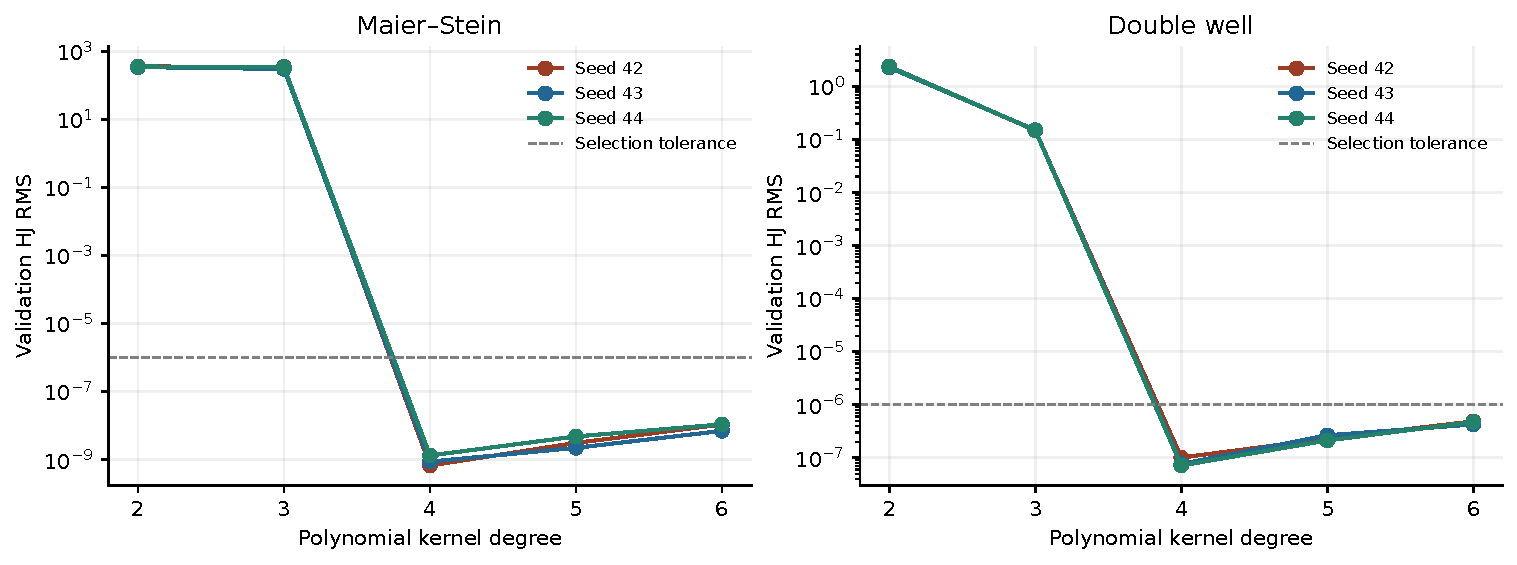
\includegraphics[width=\linewidth]{figures/native/Figure_1.pdf}
\caption{Independent validation HJ RMS versus polynomial kernel degree for three training seeds. The dashed line is the fixed selection tolerance $10^{-6}$. Both systems select the smallest acceptable degree, $r=4$.}\label{fig:pruned_kernels_vs_lambda1}
\end{figure}
\begin{figure}[htbp]\centering
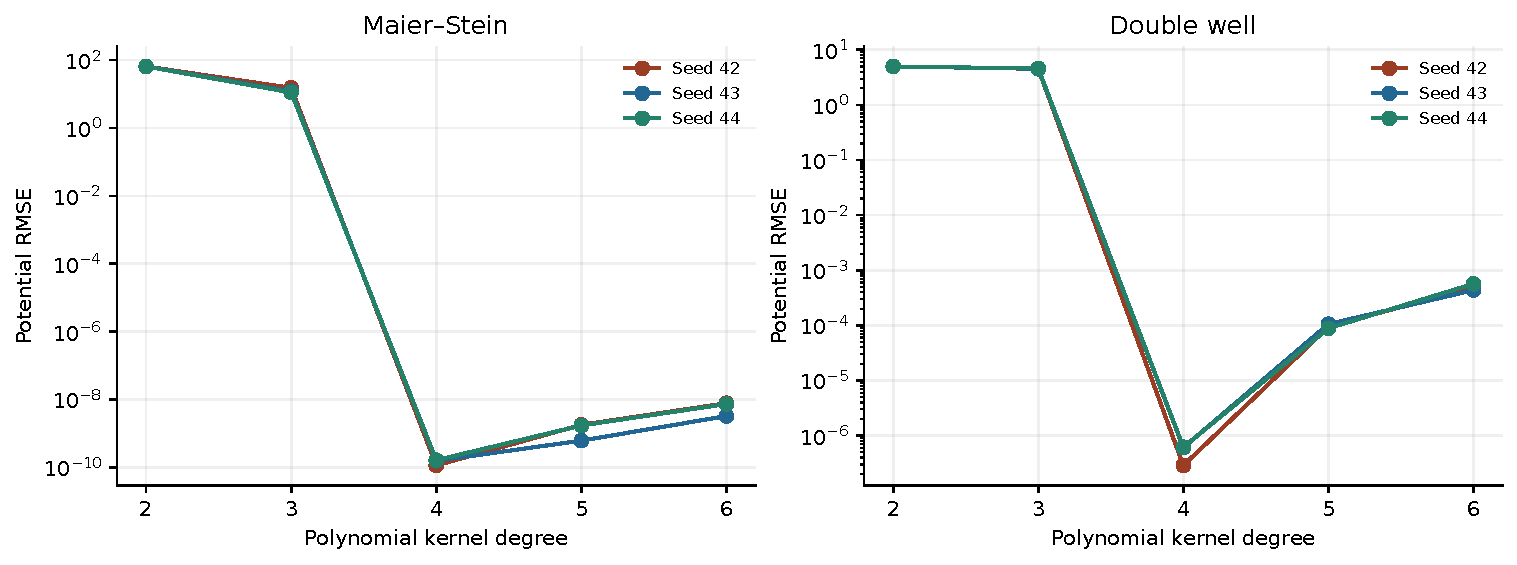
\includegraphics[width=\linewidth]{figures/native/Figure_2.pdf}
\caption{Potential RMSE for the fitted polynomial candidates. The Maier--Stein grid is $10^2$ points on $[-4,0]\times[-3,3]$; the double-well grid is $101^2$ points on $[-1.5,1.5]^2$. The latter measures error against the polynomial reference extension, including extrapolation outside the training basin. Potential errors are not used for model selection.}\label{fig:rmse_vs_lambda1}
\end{figure}
\begin{figure}[htbp]\centering
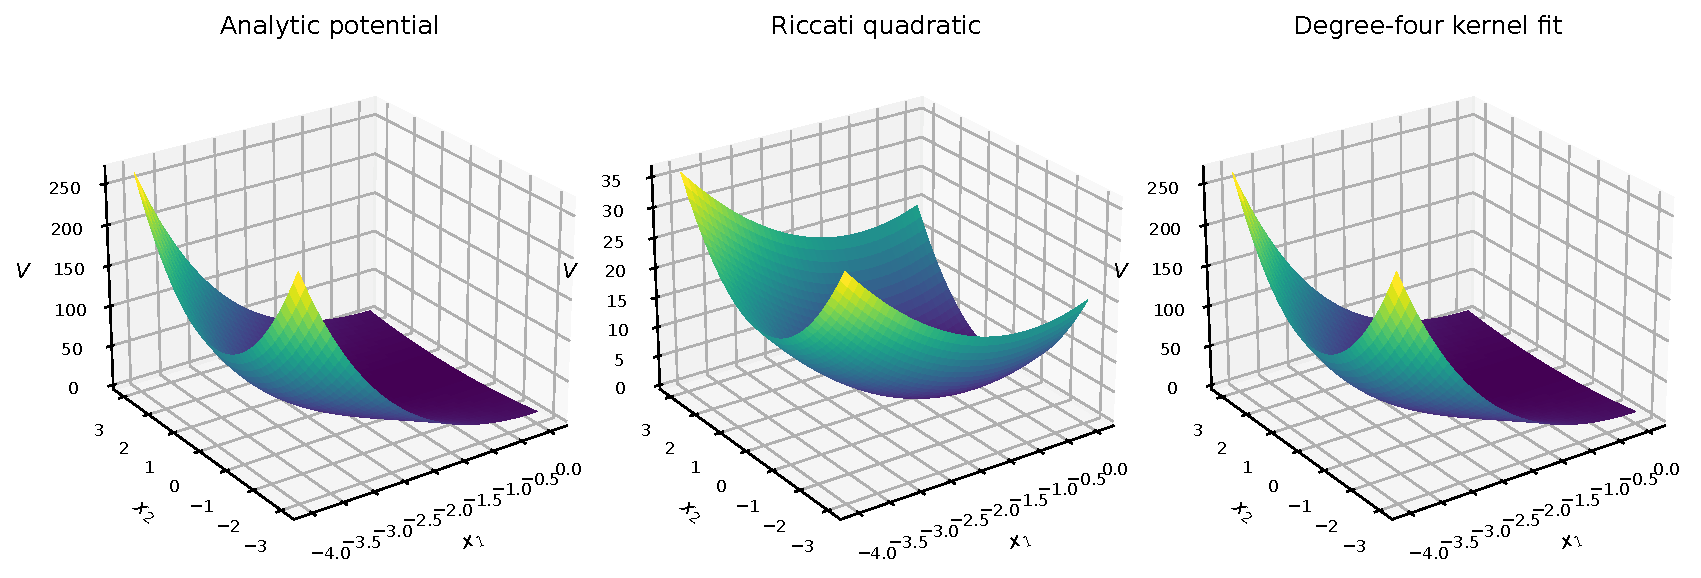
\includegraphics[width=\linewidth]{figures/native/Figure_3.pdf}
\caption{Maier--Stein potential on the left-basin closure: analytic reference, local Riccati quadratic, and the degree-four kernel fit with seed 42. Surfaces use an $81^2$ display grid; the fit uses 200 training points at each continuation radius.}\label{fig:all_V_mid_surfaces}
\end{figure}
\begin{figure}[htbp]\centering
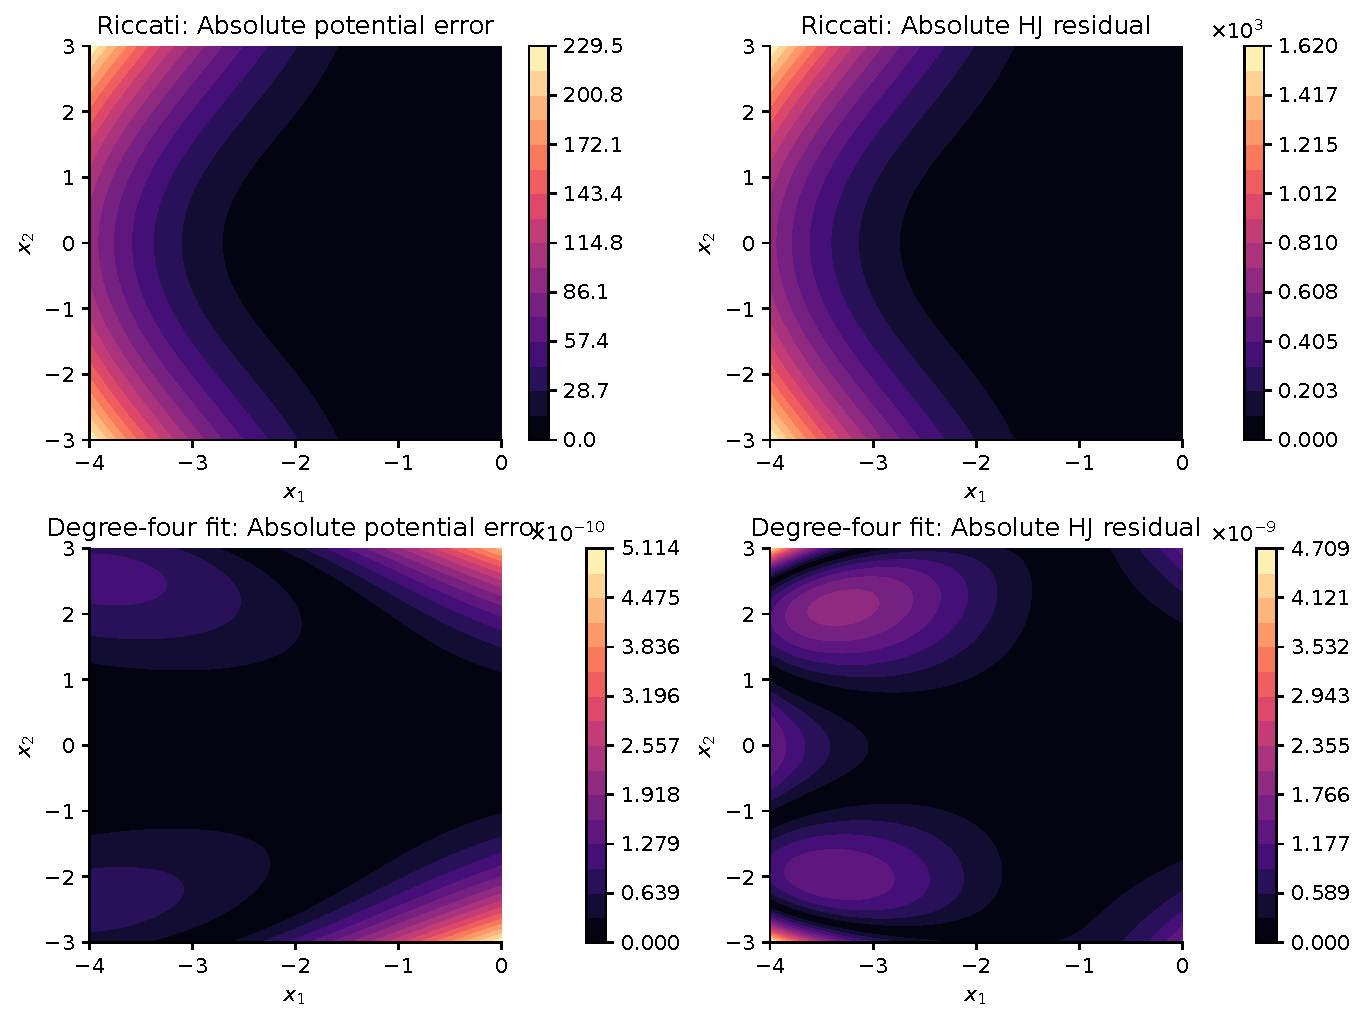
\includegraphics[width=\linewidth]{figures/native/Figure_4_residuals.pdf}
\caption{Maier--Stein absolute potential error and absolute HJ residual on the $81^2$ display grid. The top row is the Riccati baseline and the bottom row the degree-four fit. Color scales are stated separately because the errors differ by many orders of magnitude.}\label{fig:residuals_example1}
\end{figure}

\paragraph{Local constraints and interpretation.}
The representation enforces $V(\bar x)=0$, $\nabla V(\bar x)=0$, and $D^2V(\bar x)=4I$ algebraically. Accordingly, these three constraints do not rely on a finite-difference diagnostic or a penalty weight. The independent HJ checks evaluate the resulting field away from the collocation set. The example demonstrates recovery within a polynomial RKHS containing the target; general nonpolynomial systems require richer kernels and a separate assessment of approximation error.

\FloatBarrier
\subsection{Example 2: Nonlinear drift and local double-well reconstruction}\label{sec:example2_kernels}
We consider
\begin{equation}\label{sde2}
\begin{aligned}
 dx_1&=(x_1-x_1^3)\,dt+\sqrt\varepsilon\,dW_1,\\
 dx_2&=-x_2\,dt+\sqrt\varepsilon\,dW_2.
\end{aligned}
\end{equation}
The stable equilibria are $(\pm1,0)$, separated by the saddle $(0,0)$. We reconstruct the potential relative to $\bar x=(1,0)$ in the right basin. The local Jacobian is $\operatorname{diag}(-2,-1)$, so the Riccati Hessian and quadratic are
\[
 P=\begin{pmatrix}4&0\\0&2\end{pmatrix},\qquad
 V_Q(x)=2(x_1-1)^2+x_2^2.
\]
Within this basin the analytic potential is
\begin{equation}\label{eq:dw-reference}
 V_*(x)=\tfrac12(x_1^2-1)^2+x_2^2.
\end{equation}
Its continuation to $x_1<0$ is a useful polynomial reference but is not interpreted here as the global action value relative to the right-hand attractor.

\paragraph{Training and reconstruction.}
Training, validation, and independent random testing use $[0.05,1.5]\times[-1.5,1.5]$, entirely within the right basin. The continuation protocol and degree-selection rule are the same as in Example~1. Every training seed selects $r=4$. With $y_1=x_1-1$ and $y_2=x_2$, the principal fitted correction is
\[
 V_4(x)-V_Q(x)\approx 2y_1^3+\tfrac12y_1^4.
\]
Thus the selected polynomial space captures the nonlinear geometry with nine free correction coefficients. The data constrain the local well, while the reference formula permits a separate extrapolation test on a wider box.

\begin{table}[htbp]\centering
\caption{Double-well reconstruction, seed 42. Potential errors use 10,000 independent points in $[0.05,1.5]\times[-1.5,1.5]$. The level-set distance uses a separate $101^2$ grid, levels $0.1,0.2,0.3,0.4$, and band width $0.02$.}\label{tab:example2_errors}
\begin{tabular}{lccc}\toprule Method & RMSE & Relative $L^2$ & Mean $d_H$\\\midrule
Riccati & $0.413$ & $0.3423$ & $0.1317$ \\
Polynomial kernel ($r=4$) & $5.22\times10^{-8}$ & $4.33\times10^{-8}$ & $0$ \\\bottomrule\end{tabular}\end{table}


For seeds $42,43,44$, the independent-basin RMSEs are $5.22\times10^{-8}$, $4.86\times10^{-8}$, and $4.74\times10^{-8}$. The Riccati baseline has RMSE $0.4130$ on the same test set. The corresponding fitted relative errors are about $4\times10^{-8}$. On the wider $101^2$ grid over $[-1.5,1.5]^2$, the errors against the polynomial extension are $2.87\times10^{-7}$, $6.06\times10^{-7}$, and $6.17\times10^{-7}$. This separates interpolation within the training basin from extrapolation of the learned polynomial.

\paragraph{Level-set geometry.}
For each level $c$, we approximate its level set by the grid band
\[
 \Gamma_{c,h}(V)=\{x\in X_h:|V(x)-c|\leq0.02\},
\]
using a $101^2$ grid on the training box and levels $0.1,0.2,0.3,0.4$, below the saddle height $1/2$. The symmetric Hausdorff distance is computed between these finite point sets and then averaged over the four levels. The fitted and reference bands coincide on this grid, yielding zero discrete distance; this means agreement at the stated spatial and band resolution. It is not a claim of exact equality of the continuous level sets. The Riccati mean distance is approximately $0.1317$.

\paragraph{Constraint and error assessment.}
The equilibrium value, gradient, and Hessian are imposed exactly. For seed 42 the mean absolute HJ residual on the independent basin test is $6.15\times10^{-8}$ and its maximum is $6.29\times10^{-7}$. These diagnostics complement the potential error: local curvature describes the behavior near the stable point, the potential error measures the scalar reconstruction throughout the testing domain, and the level-set comparison measures its geometry. Their agreement here is facilitated by exact polynomial representability and noiseless access to the drift.

\subsection{Example 3: Multiplicative noise and quadratic reconstruction}\label{sec:example3_kernels}
Consider the three-dimensional SDE with $\rho=5$:
\begin{equation}\label{eq:example3-sde}
\begin{aligned}
 dx_1&=-x_1(1+x_1^2)\,dt+\sqrt{\varepsilon(1+x_1^2)}\,dW_1,\\
 dx_2&=(-\tfrac12x_2-\rho x_3)\,dt+\sqrt\varepsilon\,dW_2,\\
 dx_3&=(-\tfrac12x_3+\rho x_2)\,dt+\sqrt\varepsilon\,dW_3.
\end{aligned}
\end{equation}
The equilibrium is zero, the diffusion is $a(x)=\operatorname{diag}(1+x_1^2,1,1)$, and
\[
 J=\begin{pmatrix}-1&0&0\\0&-1/2&-\rho\\0&\rho&-1/2\end{pmatrix}.
\]
Solving the Lyapunov equation at zero gives $P=\operatorname{diag}(2,1,1)$. The analytic potential is exactly the Riccati quadratic,
\begin{equation}\label{eq:example3-reference}
 V_*(x)=x_1^2+\tfrac12x_2^2+\tfrac12x_3^2.
\end{equation}
The rotational terms cancel in $b\cdot\nabla V_*$, while the state-dependent diffusion cancels the nonlinear first-coordinate drift in the HJ equation. This example tests diffusion handling, normalization, and numerical stability of the kernel representation. Since the Riccati warm start is already exact, it is a consistency benchmark rather than an improvement over that baseline.

\paragraph{Anchored kernel fit.}
We use the degree-two component of the dictionary,
\[
 V_h(x)=\sum_{j=1}^{N}\alpha_j\bigl[(1+x\cdot z_j)^2-1\bigr],
\]
with centers $z_j=x_j$ drawn uniformly from $[-2,2]^3$ by seed 42. The kernel weight is one, and the subtraction enforces $V_h(0)=0$. Training minimizes
\begin{equation}\label{eq:quadratic-refit-loss}
 \frac1N\sum_{p=1}^N H(x_p,\nabla V_h(x_p))^2
 +10\|D^2V_h(0)-P\|_F^2+10^{-4}\|\alpha\|_2^2.
\end{equation}
The amplitude sparsity term is constant for this single active kernel and therefore does not affect the refit. The nine-dimensional feature parametrization in Section~\ref{sec:direct-implementation} eliminates coefficient redundancy while preserving the minimum-norm $\alpha$ and the scalar kernel function. Curvature is penalized rather than fixed in this experiment; the equilibrium gradient remains a fitted quantity. The warm start is computed from the local Lyapunov equation.

\begin{table}[htbp]\centering
\caption{Multiplicative-noise example: seed 42, $N=200$, and the fixed $20^3$ evaluation grid on $[-2,2]^3$.}\label{tab:example3_comparison}
\begin{tabular}{lccc}\toprule Method & RMSE & Maximum error & Relative $L^2$\\\midrule
Riccati & $3.67\times10^{-16}$ & $1.78\times10^{-15}$ & $1.09\times10^{-16}$ \\
Anchored kernel refit ($r=2$) & $1.35\times10^{-9}$ & $4.52\times10^{-9}$ & $4.03\times10^{-10}$ \\\bottomrule\end{tabular}\end{table}


\paragraph{Accuracy and constraints.}
At $N=200$, the fixed $20^3=8000$ point grid on $[-2,2]^3$ gives RMSE $1.35\times10^{-9}$, with the maximum and relative errors in Table~\ref{tab:example3_comparison}. The Riccati baseline remains at floating-point precision. The value anchor is exact by construction. Hessian and gradient errors, HJ residuals, and independent random-test errors are computed directly from the fitted coefficients. The supplied implementation verifies the equality of feature-space predictions and the original anchored kernel sum at independent points, as well as the analytic residual Jacobian by directional finite differences.

\paragraph{Sample-count study.}\label{sec:empirical-convergence}
We repeat the fit for $N=50,100,200,400,800$, using the same seeded sampling rule and fixed evaluation grid. The kernel-refit RMSEs are respectively $1.05\times10^{-7}$, $5.95\times10^{-9}$, $1.35\times10^{-9}$, $1.13\times10^{-9}$, and $3.88\times10^{-10}$. Every solve satisfies its gradient stopping criterion; the maximum final first-order optimality measure is below $10^{-8}$. Figure~\ref{fig:convergence_study} also gives errors on an independent set of $10000$ uniform points and the HJ residuals on both evaluation sets.

The number of identifiable polynomial coefficients is nine for all these values of $N$. Increasing $N$ changes the collocation average and the minimum-norm coefficient representation used in the ridge term. Consequently, the displayed trend describes numerical and regularization sensitivity within a fixed finite-dimensional model; no power-law approximation rate is fitted to it. The nearly exact quadratic warm start is central to this behavior.

\begin{figure}[htbp]\centering
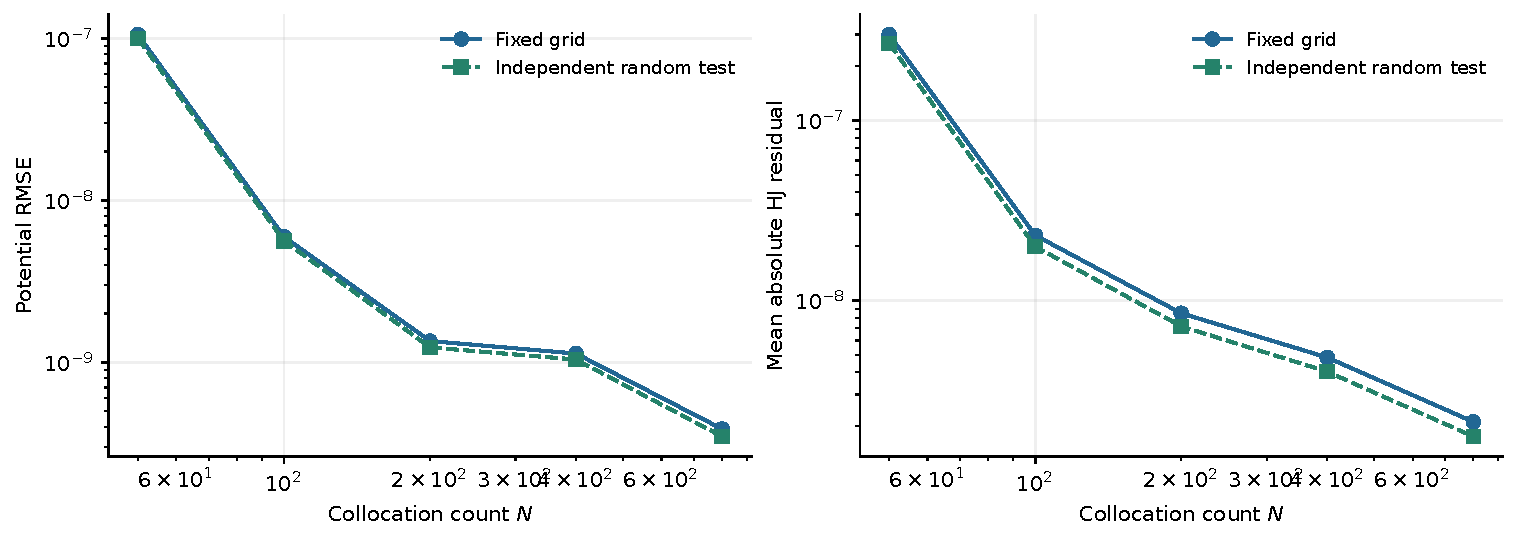
\includegraphics[width=\linewidth]{figures/native/convergence_study_example3.pdf}
\caption{Anchored degree-two kernel fits for the multiplicative-noise system. Left: potential RMSE; right: mean absolute HJ residual. The solid curves use the fixed $20^3$ grid and the dashed curves use $10000$ independent random points. Seed 42 and the same objective are used for every $N$.}\label{fig:convergence_study}
\end{figure}

\paragraph{Potential slices and spatial errors.}
Figures~\ref{fig:comparison_example3} and~\ref{fig:residuals_example3} evaluate the three coordinate planes through the equilibrium. Each plane uses an $81\times81$ grid containing zero. The displayed reference, Riccati, and fitted contours coincide visually. Absolute-error panels use separate labeled scales to resolve the kernel's small regularization bias and the Riccati baseline's rounding error. No error offset or fitted amplitude is introduced.

\begin{figure}[htbp]\centering
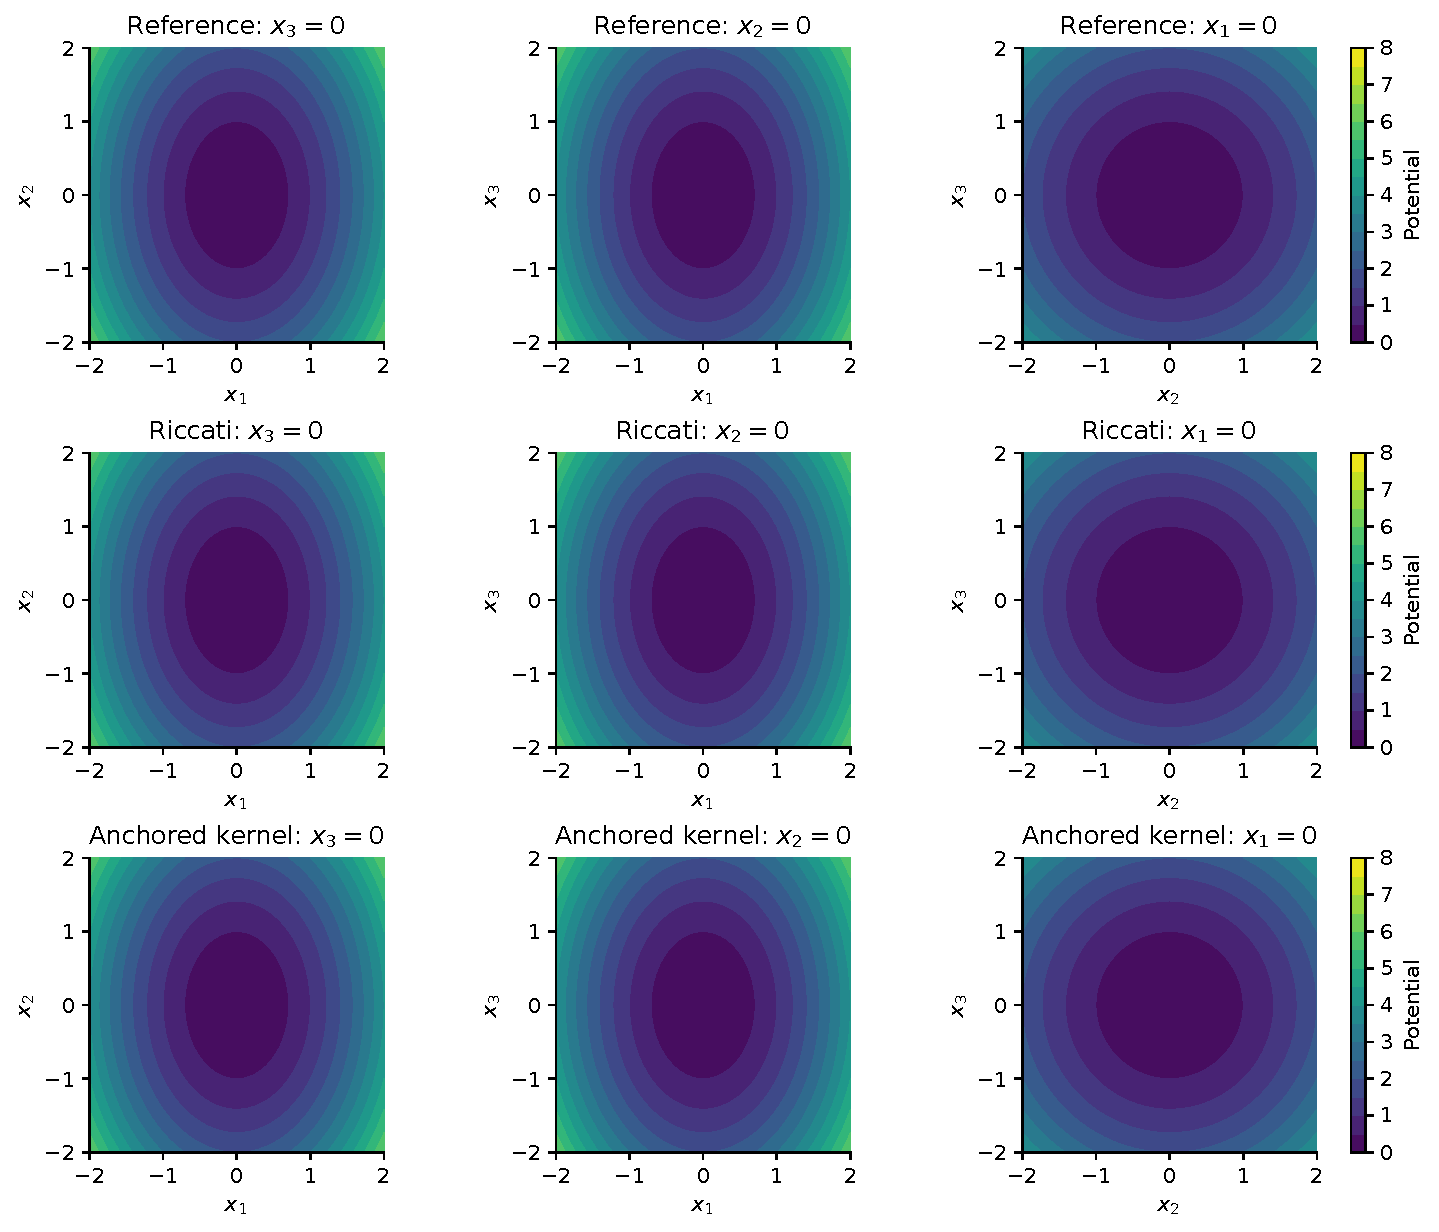
\includegraphics[width=0.95\linewidth,height=0.73\textheight,keepaspectratio]{figures/native/quasi_potential_slices_sparse.pdf}
\caption{Coordinate-plane slices of the analytic potential, Riccati baseline, and anchored degree-two kernel fit at $N=200$. Every fixed coordinate is exactly zero. A common potential range is used across all panels.}\label{fig:comparison_example3}
\end{figure}
\begin{figure}[htbp]\centering
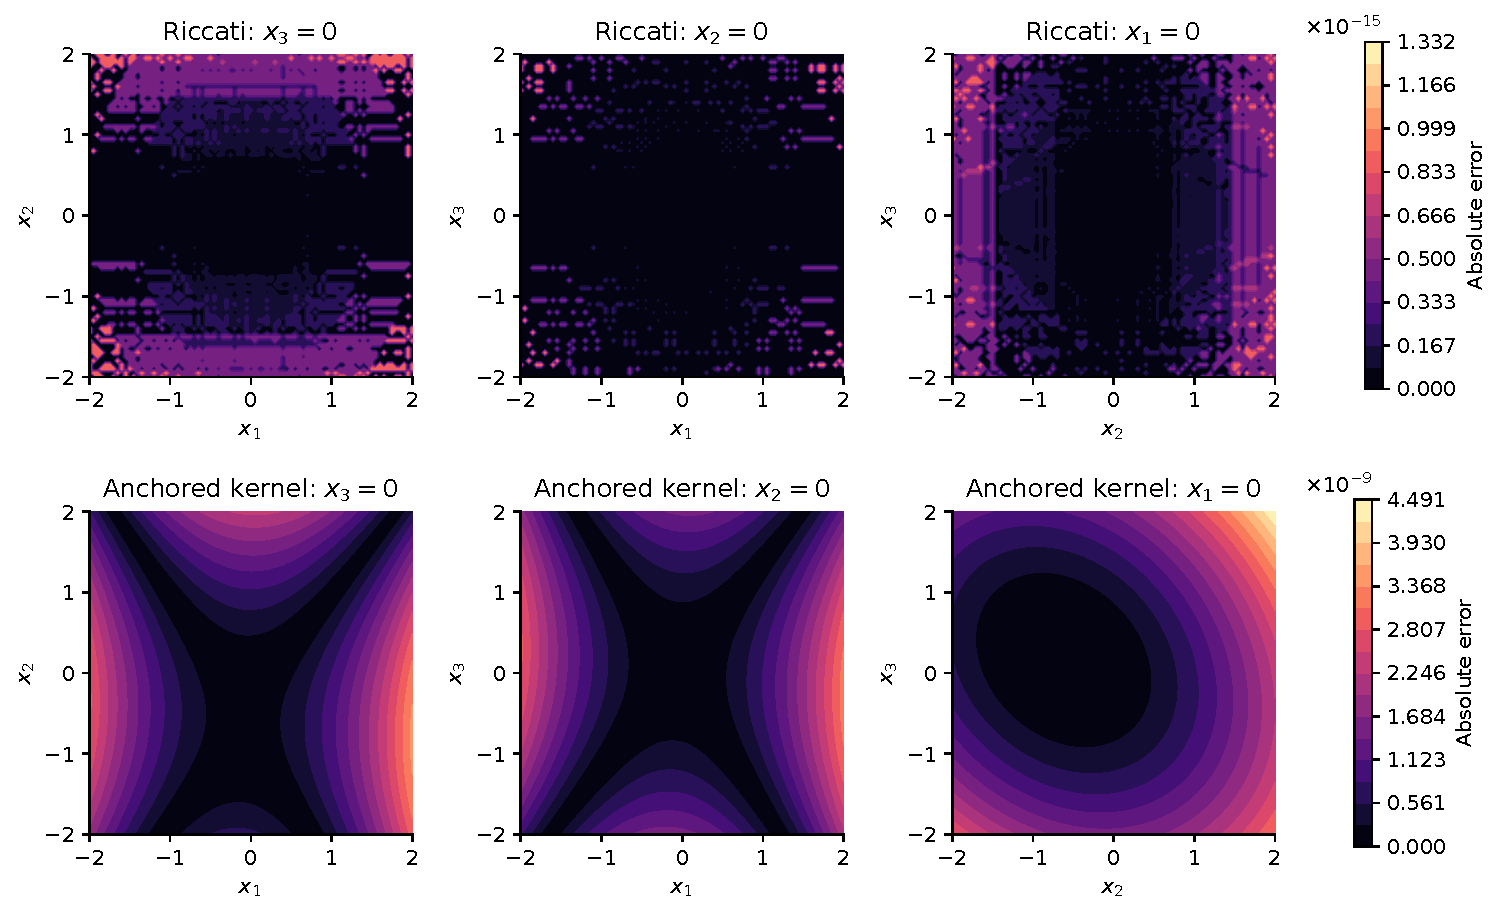
\includegraphics[width=0.95\linewidth]{figures/native/residuals_example3.pdf}
\caption{Absolute errors on the zero-coordinate slices in Figure~\ref{fig:comparison_example3}. The top row is the Riccati baseline and the bottom row the anchored kernel fit. Each row uses its own labeled error scale.}\label{fig:residuals_example3}
\end{figure}

\paragraph{Reproducibility.}
The computational package stores the training points, fitted coefficients, validation scores for every candidate, independent test points, solver termination data, and numerical derivatives. The programs \path{code/run_polynomial_experiments.py} and \path{code/refit_selected_kernel.py} generate the two-dimensional and three-dimensional fits, respectively. The program \path{code/plot_verified_experiments.py} generates all seven vector-PDF figures and both example tables directly from those results. The reference formulas are evaluated after model fitting and selection. Each figure is therefore reproducible without raster inputs or manual curve tracing.

\FloatBarrier
\section{Conclusion}

We have presented a kernel framework for quasi-potential computation with direct scalar and Koopman-coordinate representations. Both use Hamilton--Jacobi structure and local Riccati curvature. The spectral form supplies dynamical coordinates and a nonnegative quadratic surrogate, whereas direct scalar fitting avoids the additional transport restriction. Nonnegative amplitude regularization and discrete dictionary selection offer distinct controls on model complexity.

Theorem~\ref{thm:consistency-curvature} gives sufficient conditions for convergence to the selected viscosity solution. The numerical experiments recover the two-dimensional quartic benchmark potentials using degree-four kernel spaces and the multiplicative-noise quadratic using an anchored degree-two expansion. Independent validation and test points assess residuals and potential errors. Finite-feature compression stabilizes the quadratic kernel refit without changing its function class. The controlled Gaussian-kernel experiments include a structured eight-dimensional system and favor direct fitting over the tested restricted spectral candidate. These findings identify when the global representational restriction, rather than the local curvature information, controls approximation accuracy.

\paragraph{Limitations and future work.}
The main limitation of the current work is the absence of a head-to-head comparison with established methods such as ordered-upwind methods~\cite{cameron2012finding, dahiya2018ordered}, string methods~\cite{heymann2008geometric, grafke2019numerical}, and geometric minimum action approaches~\cite{zhou2008adaptive}. Such a comparison, which would require careful tuning of each method on common test problems, is left as an important direction for future work.
Dense assembly and factorization have different costs, detailed in Section~\ref{sec:complexity-full}; the present evidence does not establish a universal practical dimension cutoff; sparse collocation, reduced-order modeling, and hierarchical kernel architectures are promising mitigation strategies. Extensions to non-Gaussian or Lévy noise, globally consistent multi-basin reconstruction, and the fully data-driven setting (where drift and diffusion must themselves be estimated) also remain open.

\section*{Acknowledgments}	
The authors acknowledge support from the National Natural Science Foundation of China (Grant Nos. 12302035, 12572038, and 12372030) and Fundamental Research Funds for the Central Universities (Grant No. 30925010411).

\clearpage
\appendix
\section{Controlled comparisons and cost measurements}\label{app:additional}
\subsection{Models and fitting protocol}\label{app:protocol}
This appendix compares direct and quadratic spectral representations and measures their computational costs. Both models use a single Gaussian kernel with bandwidth selection, coefficient ridge regularization, and exact local constraints. They complement the finite polynomial-kernel implementations in Section~\ref{examples}. The restricted quadratic Koopman candidate studied here is one specific spectral model; its performance does not characterize every hybrid kernel construction.

Let $y=x-\bar x$ and $P$ be the Riccati Hessian. For kernel centers $z_j$, subtract Taylor jets at the equilibrium:
\begin{align}
 \psi_j^{(1)}(x)&=k(x,z_j)-k(\bar x,z_j)-D_1k(\bar x,z_j)y,\\
 \psi_j^{(2)}(x)&=\psi_j^{(1)}(x)-\tfrac12y^\top D_1^2k(\bar x,z_j)y.
\end{align}
These functions belong to an augmented kernel-plus-polynomial feature space. The direct scalar and restricted spectral candidates are
\begin{align}\label{eq:appendix-models}
 V_D(x)&=\tfrac12y^\top Py+\sum_{j=1}^M c_j\psi_j^{(2)}(x),\\
 \Phi(x)&=y+\sum_{j=1}^M c_j^K\psi_j^{(1)}(x),\qquad
 V_K(x)=\tfrac12\Phi(x)^\top P\Phi(x).
\end{align}
Both satisfy $V(\bar x)=0$, $\nabla V(\bar x)=0$, and $D^2V(\bar x)=P$ exactly. $V_K$ is nonnegative; global nonnegativity of $V_D$ is not automatic. The direct coefficients minimize mean squared HJ residual plus $10^{-8}\|c\|_2^2$. The spectral coefficients minimize the mean squared real vector transport residual $\|D\Phi\,b-F\Phi\|_2^2$ plus $10^{-8}\|C_K\|_F^2$. The latter is linear least squares in $Mn$ coefficients. The Euclidean coefficient penalty differs from the RKHS norm defined by the kernel Gram matrix.

For each system and each seed in $\{230923,230924,230925\}$, the methods share $N=256$ independent uniform training points, $512$ validation points, $4096$ test points, and the first $M=32$ training points as centers. The kernel is Gaussian with $\ell/\sqrt n\in\{0.5,1,2\}$. Each method chooses its bandwidth by the smallest validation HJ residual; reference potential values never enter fitting or selection. Direct nonlinear least squares starts at the Riccati quadratic, uses an analytic Jacobian, tolerances $10^{-10}$, and a $200$-evaluation limit. The spectral fit uses the real coupled linear system. All candidate solves terminated successfully; the largest observed nonlinear evaluation count was $54$. The comparison uses common data and constraints, but not equal parameter counts or identical fitting objectives.

\subsection{Domains, higher-dimensional example, and results}\label{app:accuracy}
The first three systems use the drift and diffusion coefficients in Section~\ref{examples}, with local testing boxes $[-1.5,-0.5]\times[-0.6,0.6]$ for Example~1, $[0.5,1.5]\times[-0.6,0.6]$ for Example~2, and $[-1,1]^3$ for Example~3. These local domains and Gaussian fitting protocols differ from the polynomial-kernel experiments in Section~\ref{examples}. Example~3's Riccati quadratic is exact and is the direct model's starting point; its direct result is therefore a consistency check, not a learned improvement over Riccati.

The eight-dimensional system is defined by
\begin{equation}\label{eq:appendix-eight}
 V_*(x)=\sum_{i=1}^8(x_i^2+0.1x_i^4),\quad
 b=-\tfrac12\nabla V_*+R\nabla V_*,\quad a=I,
\end{equation}
with $R_{i,i+1}=1/4$, $R_{i+1,i}=-1/4$ and all other entries zero, on $[-1,1]^8$. Its equilibrium is zero, $F=-I+2R$ is Hurwitz, and $P=2I$. Skew symmetry gives $H(x,\nabla V_*)=0$. Completion of squares in the action gives $S_T\geq V_*(x)-V_*(0)$; the uphill flow $\dot x=\nabla V_*/2+R\nabla V_*$ attains equality in the infinite-time limit. Its reverse decreases the coercive $V_*$ strictly away from zero and converges to zero, which identifies the action value through truncation near the equilibrium. The drift is nonlinear and non-gradient, but the potential is separable, so this is a structured stress test rather than general high-dimensional validation.

\begin{table}[htbp]
\centering\small
\caption{Test errors: mean $\pm$ sample standard deviation over three seeds. No reference-based rescaling is applied. MS, DW, Mult., and Rot. identify the four test systems.}\label{tab:accuracy}
\begin{tabular}{@{}llccc@{}}
\toprule
Example & Model & RMSE & Relative $\ell^2$ error & HJ RMS\\
\midrule
1: MS, $d=2$ & Riccati & \shortstack{$0.173$\\{\scriptsize$\pm 0.00285$}} & \shortstack{$0.326$\\{\scriptsize$\pm 0.00182$}} & \shortstack{$1.05$\\{\scriptsize$\pm 0.0187$}}\\
 & Direct & \shortstack{$0.00189$\\{\scriptsize$\pm 3.10\!\times\!10^{-4}$}} & \shortstack{$0.00355$\\{\scriptsize$\pm 5.41\!\times\!10^{-4}$}} & \shortstack{$0.00868$\\{\scriptsize$\pm 8.01\!\times\!10^{-4}$}}\\
 & Koopman & \shortstack{$0.893$\\{\scriptsize$\pm 0.0512$}} & \shortstack{$1.68$\\{\scriptsize$\pm 0.119$}} & \shortstack{$33.6$\\{\scriptsize$\pm 4.68$}}\\
\addlinespace
2: DW, $d=2$ & Riccati & \shortstack{$0.0952$\\{\scriptsize$\pm 0.00108$}} & \shortstack{$0.261$\\{\scriptsize$\pm 0.00109$}} & \shortstack{$0.574$\\{\scriptsize$\pm 0.00729$}}\\
 & Direct & \shortstack{$0.0438$\\{\scriptsize$\pm 0.0344$}} & \shortstack{$0.121$\\{\scriptsize$\pm 0.0953$}} & \shortstack{$0.026$\\{\scriptsize$\pm 0.00843$}}\\
 & Koopman & \shortstack{$0.414$\\{\scriptsize$\pm 0.0728$}} & \shortstack{$1.13$\\{\scriptsize$\pm 0.186$}} & \shortstack{$13.1$\\{\scriptsize$\pm 4.3$}}\\
\addlinespace
3: Mult., $d=3$ & Riccati & \shortstack{$8.60\!\times\!10^{-17}$\\{\scriptsize$\pm 1.22\!\times\!10^{-18}$}} & \shortstack{$1.13\!\times\!10^{-16}$\\{\scriptsize$\pm 8.75\!\times\!10^{-19}$}} & \shortstack{$1.10\!\times\!10^{-15}$\\{\scriptsize$\pm 3.10\!\times\!10^{-17}$}}\\
 & Direct & \shortstack{$8.60\!\times\!10^{-17}$\\{\scriptsize$\pm 1.22\!\times\!10^{-18}$}} & \shortstack{$1.13\!\times\!10^{-16}$\\{\scriptsize$\pm 8.75\!\times\!10^{-19}$}} & \shortstack{$1.10\!\times\!10^{-15}$\\{\scriptsize$\pm 3.10\!\times\!10^{-17}$}}\\
 & Koopman & \shortstack{$0.195$\\{\scriptsize$\pm 0.0207$}} & \shortstack{$0.256$\\{\scriptsize$\pm 0.0286$}} & \shortstack{$0.351$\\{\scriptsize$\pm 0.0145$}}\\
\addlinespace
4: Rot., $d=8$ & Riccati & \shortstack{$0.177$\\{\scriptsize$\pm 5.96\!\times\!10^{-4}$}} & \shortstack{$0.0595$\\{\scriptsize$\pm 1.07\!\times\!10^{-4}$}} & \shortstack{$0.71$\\{\scriptsize$\pm 0.00251$}}\\
 & Direct & \shortstack{$0.0411$\\{\scriptsize$\pm 1.86\!\times\!10^{-4}$}} & \shortstack{$0.0138$\\{\scriptsize$\pm 5.07\!\times\!10^{-5}$}} & \shortstack{$0.147$\\{\scriptsize$\pm 0.0051$}}\\
 & Koopman & \shortstack{$0.485$\\{\scriptsize$\pm 0.00386$}} & \shortstack{$0.163$\\{\scriptsize$\pm 0.00162$}} & \shortstack{$1.46$\\{\scriptsize$\pm 0.00471$}}\\
\bottomrule
\end{tabular}
\end{table}


Table~\ref{tab:accuracy} reports means and sample standard deviations across three seeds. Relative error is $\|u-V\|_{\ell^2(X_t)}/\|V\|_{\ell^2(X_t)}$; HJ RMS is the root mean squared residual on the independent test points. The direct model is more accurate than the restricted spectral candidate in all four tests. The double-well direct fit has appreciable seed variability, as shown by the tabulated standard deviation. The eight-dimensional mean relative errors are approximately $5.95\%$ for Riccati, $1.38\%$ for direct fitting, and $16.31\%$ for the spectral candidate. These comparisons do not establish universal model rankings, a viscosity convergence certificate, or certified escape-barrier accuracy. They show why Koopman features should be treated as an optional restriction, rather than presumed to improve a direct fit.

\begin{figure}[htbp]
\centering
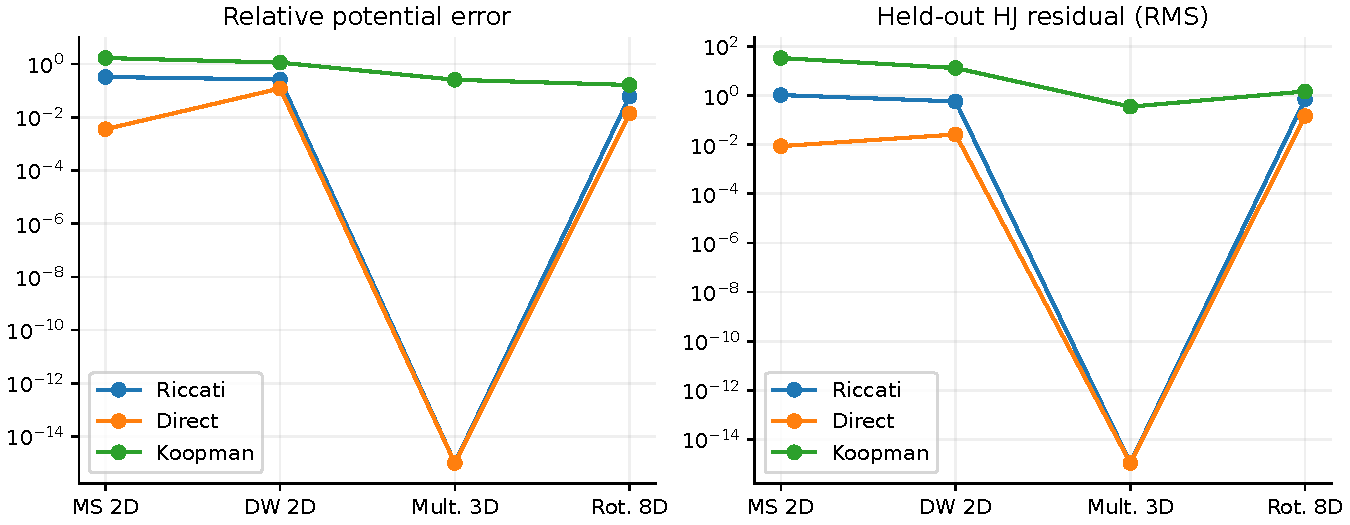
\includegraphics[width=\textwidth]{figures/ablation.pdf}
\caption{Controlled model comparison: mean relative potential error and independent-test HJ RMS over three seeds. MS, DW, Mult., and Rot. denote the Maier--Stein, double-well, multiplicative-noise, and eight-dimensional rotational systems. Values below $10^{-15}$ are drawn at $10^{-15}$ for visibility. All fits use the single-kernel protocol of Appendix~\ref{app:protocol}.}\label{fig:additional-ablation}
\end{figure}

\subsection{Runtime, memory accounting, and reproducibility}\label{app:runtime}
\begin{table}[htbp]
\centering\small
\caption{Median measured time in milliseconds. Fit includes the three-bandwidth search and validation; test is value and gradient prediction on 4096 points. Problem setup, imports, plots, and error calculation are excluded.}\label{tab:timing}
\begin{tabular}{@{}lrrrrr@{}}
\toprule
 & \multicolumn{2}{c}{Direct} & \multicolumn{2}{c}{Koopman} & Riccati\\
Example & Fit & Test & Fit & Test & Test\\
\midrule
1: MS, $d=2$ & 30.17 & 7.81 & 3.70 & 5.29 & 0.11\\
2: DW, $d=2$ & 22.13 & 6.12 & 3.46 & 5.05 & 0.12\\
3: Mult., $d=3$ & 4.87 & 7.70 & 5.09 & 6.56 & 0.16\\
4: Rot., $d=8$ & 19.79 & 20.05 & 14.34 & 13.96 & 0.41\\
\bottomrule
\end{tabular}
\end{table}

\begin{table}[htbp]
\centering\small
\caption{Dense Gaussian Gram microbenchmark: median milliseconds after one warm-up, with storage for the Gram matrix alone. MiB denotes $2^{20}$ bytes. This is separate from the reduced-center fits.}\label{tab:dense}
\begin{tabular}{@{}rrrrr@{}}
\toprule
$d$ & $N$ & Assembly (ms) & Cholesky (ms) & Gram (MiB)\\
\midrule
2 & 128 & 0.105 & 0.037 & 0.125\\
2 & 256 & 0.277 & 0.271 & 0.500\\
2 & 512 & 1.731 & 1.748 & 2.000\\
2 & 1024 & 11.383 & 8.923 & 8.000\\
8 & 128 & 0.108 & 0.044 & 0.125\\
8 & 256 & 0.288 & 0.285 & 0.500\\
8 & 512 & 1.723 & 1.721 & 2.000\\
8 & 1024 & 12.268 & 10.436 & 8.000\\
\bottomrule
\end{tabular}
\end{table}


Table~\ref{tab:timing} measures fitting/selection over all three bandwidths and value/gradient prediction at $4096$ test points. Initial model/Lyapunov setup, imports, plots, and reference-error calculation are excluded. Table~\ref{tab:dense} separately measures Gaussian Gram assembly and Cholesky factorization, using $10^{-6}I$ regularization and medians of three repeats after one warm-up. It is not a timing of the complete PDE solver. Gram storage is $8N^2$ bytes; peak process memory was not measured and would also include factors, distances, derivatives, and optimization work arrays. A single $6400\times6400$ float64 matrix already occupies $312.5$ MiB.

The recorded environment is CPU float64 on macOS 15.8 ARM64, Python 3.12.14, NumPy 2.5.3, SciPy 1.18.1, and Matplotlib 3.11.2. Single-thread limits were requested through environment variables and \texttt{threadpoolctl}; no inspectable pools were reported, so the vendor thread count was not independently confirmed. Short timings depend on system load and caching. Four matrix sizes do not establish a measured asymptotic complexity exponent.

The computational archive contains \path{code/run_experiments.py}, which defines the systems, derivatives, seeds, data splits, and solvers for the controlled comparisons. It checks gradients and equilibrium Hessians by finite differences and verifies the analytic HJ/Riccati identities and coupled transport assembly before fitting. The file \path{results/experiments.json} contains all 36 method/seed outcomes, candidate diagnostics, and timing/environment metadata, while \path{results/fitted_models.npz} stores coefficients, centers, and plotted grids. The scripts \path{code/make_tables.py} and \path{code/generate_figures.py} produce the tables and vector-PDF comparison plots from saved results. These materials support reproduction of the Gaussian-kernel comparisons. The main-text polynomial experiments are generated by \path{code/run_polynomial_experiments.py} and \path{code/refit_selected_kernel.py}; their saved inputs and outputs are in \path{results/accuracy/}. The program \path{code/plot_verified_experiments.py} generates the seven main-text figures and two numerical tables.

\FloatBarrier

\bibliographystyle{abbrv}
\bibliography{references_full_revision}

\end{document}
